%\documentclass[handout]{beamer}%no animations
\documentclass{beamer}%with animations
\synctex=1
%\pdfoutput = 1
%\usepackage[english,danish]{babel}
%\usepackage[applemac]{inputenc}
%\usepackage{qtree}
\usepackage{hyperref}
\usepackage{mibmrcfg}
\usepackage{amscd}
%\usepackage{proof}
\usepackage{multirow}
\usepackage{tabularx}
%\usepackage{ifpdf}


\newcommand{\miqed}{\qed}

\usepackage[normalem]{ulem}

\usepackage{ifpdf}
\usepackage{ifthen}

\ifpdf
  \newcommand{\inputfig}[1]{
    %\includegraphics[angle=-90]{#1.pdftex}
    \input{#1.pdftex_t}
  }
%  \DeclareGraphicsRule{.pdftex}{pdf}{.pdftex}{}
\else
  \newcommand{\inputfig}[1]{\input{#1.pstex_t}}
\fi

\newcommand{\tsigma}{\mathcal{T}_{\Sigma}} 
\newcommand{\tsigmav}{\tsigma(\Var)}

\newcommand{\crypt}[2]{\{#2\}_{#1}}
\newcommand{\scrypt}[2]{\{\!| #2 |\!\}_{#1}}
\newcommand{\inv}[1]{\iffont{inv}(#1)}
\newcommand{\pair}[2]{\langle #1, #2 \rangle}
%\newcommand{\fst}[1]{\pi_1(#1)}
%\newcommand{\snd}[1]{\pi_2(#1)}
\newcommand{\tuple}[1]{\langle #1 \rangle}

\newcommand{\idfont}[1]{\mathit{#1}}
\newcommand{\HN}{\idfont{HN}}
\newcommand{\NA}{\idfont{NA}}
\newcommand{\NB}{\idfont{NB}}
\newcommand{\na}{\idfont{na}}
\newcommand{\nb}{\idfont{nb}}
\newcommand{\GX}{\idfont{GX}}
\newcommand{\GY}{\idfont{GY}}

\newcommand{\pkNA}{\iffont{pk}}
\newcommand{\skNA}{\iffont{sk}}
\newcommand{\pk}[1]{\pkNA(#1)}
\newcommand{\sk}[1]{\skNA(#1)}

\newcommand{\dyS}{\mathcal{DY}}
\newcommand{\dy}[1]{\dyS(#1)}
\newcommand{\dym}[2]{\dyS_{#1}(#2)}
\newcommand{\dymS}[1]{\dyS_{#1}}
\newcommand{\public}{\Sigma_p}
%{\mathit{public}}

\newcommand{\state}[2]{\stateNA_{#1}(#2)}
\newcommand{\stateNA}{\iffont{state}}
\newcommand{\iknows}[1]{\iknowsNA(#1)}
\newcommand{\iknowsNA}{\iffont{iknows}}
%\newcommand{\knows}[2]{\iffont{knows}(#1,#2)}
\newcommand{\ifnot}[1]{\iffont{not}(#1)}
\newcommand{\ifdot}{{}_{\;\bullet\;}}

\newcommand{\ifarrow}[1][]{
  \ifthenelse{\equal{#1}{}}{
    \Rightarrow
  }{
    =\!\!\![{#1}]\!\!\!\hspace{1pt}\Rightarrow
  }}

\newcommand{\iffont}[1]{\mathsf{#1}}

\newcommand{\roleA}{\mathcal{A}}
\newcommand{\roleB}{\mathcal{B}}
\newcommand{\roleR}{\mathcal{R}}

%\newcommand{\drightarrow}{\rightarrow\!\!\!\!\!\rightarrow}

\newcommand{\secCh}{\mbox{$\,\bullet\!\!\rightarrow\!\!\bullet\,$}}
\newcommand{\athCh}{\mbox{$\,\bullet\!\!\rightarrow$\,}}
\newcommand{\cnfCh}{\mbox{${\rightarrow\!\!\bullet\,}$}}
% \newcommand{\secChRP}{\,\bullet\!\!\!\drightarrow\!\!\bullet\,}
% \newcommand{\athChRP}{\,\bullet\!\!\!\drightarrow}
% \newcommand{\cnfChRP}{\drightarrow\!\!\bullet\,}
\newcommand{\secRCh}{\,\bullet\!\!\!\twoheadrightarrow\!\!\bullet\,}
\newcommand{\athRCh}{\,\bullet\!\!\!\twoheadrightarrow}
\newcommand{\insecCh}{\rightarrow}

\newcommand{\onionCh}{\,\bullet[\rightarrow]\bullet\,}

\newcommand{\idmxCh}{\onionCh}

\newcommand{\dotChdot}{\,\bullet\!\!\leftrightarrow\!\!\bullet\,}
\newcommand{\dotCh}{\,\bullet\!\!\leftrightarrow}
\newcommand{\Chdot}{\leftrightarrow\!\!\bullet\,}

\newcommand{\PsecChP}{\,\circ\!\!\!\rightarrow\!\!\circ\,}
\newcommand{\PsecCh}{\,\circ\!\!\!\rightarrow\!\!\bullet\,}
\newcommand{\secChP}{\,\bullet\!\!\!\rightarrow\!\!\circ\,}
\newcommand{\PathCh}{\,\circ\!\!\!\rightarrow}
\newcommand{\cnfChP}{\rightarrow\!\!\circ\,}

\newcommand{\PChP}{\,\circ\!\!\leftrightarrow\!\!\circ\,}
\newcommand{\dotChP}{\,\bullet\!\!\leftrightarrow\!\!\dot\,}
\newcommand{\PChdot}{\,\circ\!\!\leftrightarrow\!\!\bullet\,}
\newcommand{\PCh}{\,\circ\!\!\leftrightarrow}
\newcommand{\ChP}{\leftrightarrow\!\!\circ\,}

% \newcommand{\FsecCh}[3]{\iffont{secCh}_{#1,#2}(#3)}
% \newcommand{\FathCh}[2]{\iffont{athCh}_{#1}(#2)}
% \newcommand{\FcnfCh}[2]{\iffont{cnfCh}_{#1}(#2)}

\newcommand{\athIssue}[1]{\iffont{athIssue(#1)}}
\newcommand{\cnfIssue}[1]{\iffont{cnfIssue(#1)}}
\newcommand{\secIssue}[1]{\iffont{secIssue(#1)}}
\newcommand{\athRely}[1]{\iffont{athRely(#1)}}
\newcommand{\cnfRely}[1]{\iffont{cnfRely(#1)}}
\newcommand{\secRely}[1]{\iffont{secRely(#1)}}

\newcommand{\pkEnc}[1]{\mathit{pkEnc}(#1)}
\newcommand{\pkSig}[1]{\mathit{pkSig}(#1)}

\newcommand{\DownGrade}{\mathrm{DownGrade}}
\newcommand{\Combine}{\mathrm{Combine}}
\newcommand{\SymOne}{\mathrm{Sym_1}}
\newcommand{\SymTwo}{\mathrm{Sym_2}}
\newcommand{\SymTre}{\mathrm{Sym_3}}
\newcommand{\CreatePseudo}{\mathrm{CreatePseudo}}
\newcommand{\UsePseudo}{\mathrm{UsePseudo}}
\newcommand{\UseRealName}{\mathrm{UseRealName}}
\newcommand{\PseudoDownGrade}{\mathrm{PseudoDownGrade}}
\newcommand{\AuthPseudo}{\mathrm{AuthPseudo}}
\newcommand{\AthTTP}{\mathrm{AthTTP}}
\newcommand{\CnfTTP}{\mathrm{CnfTTP}}
\newcommand{\SecTTP}{\mathrm{SecTTP}}


\newcommand{\honest}[1]{\mathit{honest}(#1)}
\newcommand{\dishonest}[1]{\iffont{dishonest}(#1)}
\newcommand{\vddash}{\vdash\!\!\!\vdash}
\newcommand{\mmodels}{\models\hspace{-0.3cm}\models}

\newcommand{\IK}{\mathit{IK}}
\newcommand{\agent}[1]{\iffont{agent}(#1)}

\newcommand{\Fresh}{\mathit{Fresh}}
\newcommand{\Payload}{\mathit{Payload}}
\newcommand{\Public}{\mathit{Public}}
\newcommand{\Tag}{\mathit{Tag}}
\newcommand{\lift}[1]{\lceil #1\rceil}

\newcommand{\pos}[1]{\mathit{pos}(#1)}
\newcommand{\Var}{\mathcal{V}}

\newcommand{\tagfont}[1]{\mathsf{#1}}
\newcommand{\tSone}{\tagfont{S_1}}
\newcommand{\tStwo}{\tagfont{S_2}}

\newcommand{\optfix}[2][]{}
%{{\fbox{opt}}} 
%{\bf FIX}\footnote{{\bf FIX: #1}: #2}}
%\newcommand{\fix}[2][]{{\bf FIX}\footnote{{\bf FIX #1}: #2}}

\newcommand{\dyM}[2]{\mathcal{DY}_{#1}(#2)}
\newcommand{\nf}[1]{#1_{\downarrow C/F}}
\newcommand{\pattern}[2]{{\lceil\,#1\,\rceil}_{#2}}
\newcommand{\decryptPat}[2]{{\lceil\!\!\lceil\,#1\,\rceil\!\!\rceil}_{#2}}

\newcommand{\pubNA}{\mathit{pub}}
\newcommand{\responseNA}{\mathit{response}}
\newcommand{\checkRNA}{\mathit{check}}

\newcommand{\pub}[1]{\pubNA(#1)}
\newcommand{\response}[1]{\responseNA(#1)}
\newcommand{\checkR}[1]{\checkRNA(#1)}

\newenvironment{AnB}
{ %\begin{minipage}{\linewidth}
$ %      \begin{displaymath}
        % \renewcommand{\arraystretch}{1.2}
        \begin{array}{l}
        }
        {\end{array}
        % \renewcommand{\arraystretch}{1}
$ %      \end{displaymath}
    %\end{minipage}
  }

\newcommand{\keyword}[1]{\mathtt{#1}}

\newcommand{\Protocol}[5]{
  \keyword{Protocol:}~\mathit{#1}\\
  \keyword{Types:}\\
  #2
  \keyword{Knowledge:}\\
  #3
  \keyword{Actions:}\\
  \begin{array}{ccccl}
  #4
  \end{array}\\
  \keyword{Goals:}\\
  \begin{array}{ccccl}
  #5
  \end{array}
}
\newcommand{\MidProtocol}[5]{
%   \keyword{Knowledge:}\\
%   #3
%   \keyword{Actions:}\\
  \begin{array}{ccccl}
  #4
  \end{array}\\
}

\newcommand{\MSC}[5]{
  \keyword{Protocol:}~\mathit{#1}\\
  \begin{array}{ccccl}
    #4
  \end{array}
}

\newcommand{\ShortProtocol}[5]{
  \keyword{Protocol:}~\mathit{#1}\\
  %\ldots\\
  %\keyword{Actions:}\\
  \begin{array}{ccccl}
  #4
\end{array}\\
%\ldots
}
\newcommand{\CompactProtocol}[5]{
  %\keyword{Protocol:}~\mathit{#1}\\
  %\ldots\\
  %\keyword{Actions:}\\
  \begin{array}{ccccl}
  #4
  \hline
  #5
  \end{array}\\
%\ldots
}
\newcommand{\Type}[2]{\quad #1\;\mathit{#2};\\}
\newcommand{\Agent}{\keyword{Agent}}
\newcommand{\Number}{\keyword{Number}}
\newcommand{\Function}{\keyword{Function}}
\newcommand{\TFunction}{\keyword{Function}}
\newcommand{\Knowledge}[2]{\quad\mathit{#1}:~\mathit{#2};\\}
\newcommand{\Create}[2]{
  \multicolumn{5}{l}{\quad\#\mathit{#1}~\text{creates}~\mathit{#2}}\\}
\newcommand{\Let}[2]{
  \multicolumn{5}{l}{\quad\#\mathit{#1}~:=~\mathit{#2}}\\}
\newcommand{\Action}[4]{\quad\mathit{#1}&#2&\mathit{#3}&:&\mathit{#4}\\}
\newcommand{\Repeat}[5]{\multicolumn{5}{l}{
    \quad#1=\mathit{#2}#3\mathit{#4}:\mathit{#5}}\\}
\newcommand{\NGoal }[4]{\quad\mathit{#1}&#2&\mathit{#3}&:&\mathit{#4}\\}
\newcommand{\AuthGoal}[3]
{\multicolumn{5}{l}{
    \quad\mathit{#1}~\keyword{authenticates}~\mathit{#2}~%
    \keyword{on}~\mathit{#3}}\\}
\newcommand{\SecGoal}[2]
{\multicolumn{5}{l}{\quad\mathit{#1}~\keyword{secret~of}~\mathit{#2}}\\}
\newcommand{\REML}[1]{\multicolumn{5}{l}{\quad\#\text{ #1}}\\}

% \newenvironment{IF}
% {\begin{displaymath}\begin{array}[c]{l}}
% {\end{array}\end{displaymath}}

\newcommand{\ifrule}[3]{#1\\ \ifarrow[#2]\\ #3\\[2ex]}

\newcommand{\subterm}{\sqsubseteq}
\newcommand{\propersubterm}{\sqsubset}
\newcommand{\supterm}{\sqsupseteq}
\newcommand{\propersupterm}{\sqsupset}

\newcommand{\decryptions}[2]{\mathit{decryptions}_{#1}(#2)}
\newcommand{\patternR}[3]{\pattern{#2}{#3}^{#1}}

\newcommand{\instanceof}{\succeq}

\newcommand{\secret}[2]{\iffont{secret}(#1,#2)}

\newcommand{\idemix}{\textsf{Identity Mixer}}

\newcommand{\xor}{\oplus}
\newcommand{\algo}[1]{\ensuremath{\mathsf{#1}}}
\newcommand{\const}[1]{\algo{#1}}
\newcommand{\vari}[1]{\ensuremath{\mathit{#1}}}

\newcommand{\ana}[2]{\mathit{ana}_{#1}(#2)}
\newcommand{\derivations}[3]{\mathit{derivations}_{#1}(#2,#3)}
\newcommand{\dereq}[3]{\mathit{dereq}_{#1}(#2,#3)}
\newcommand{\checks}[3]{\mathit{checks}_{#1}(#2,#3)}
\newcommand{\given}[1]{\textsl{given}(#1)}
\newcommand{\ungive}[1]{{#1}_*}

%% Declare COLORS
%% ============================
\definecolor{grey}{rgb}{0.8,0.8,0.8}\newcommand{\grey}{\color{grey}}
\definecolor{red}{rgb}{1,0,0}\newcommand{\red}{\color{red}}
\definecolor{green}{rgb}{0,0.45,0}\newcommand{\green}{\color{green}}
\definecolor{blue}{rgb}{0,0,1}\newcommand{\blue}{\color{blue}}

\newcommand{\rpif}{\mathbb{P}}
\newcommand{\rif}{\mathbb{R}}
\newcommand{\rf}{\mathbb{F}}
%\newcommand{\re}{\mathbb{E}}
\newcommand{\md}{\mathbb{M}}
\newcommand{\traces}{\mathbb{T}}
\newcommand{\sigS}{\iffont{pk}(S)}
\newcommand{\send}[2]{\iffont{snd}_{#1}(#2)}
\newcommand{\recv}[2]{\iffont{rcv}_{#1}(#2)}
\newcommand{\trace}{t}
\newcommand{\evs}{\mathit{evs}}
\newcommand{\evt}{\mathit{evt}}
\newcommand{\mkset}[1]{[#1]} %\mathit{mkset}(#1)}
\newcommand{\player}[1]{\mathit{player}(#1)}
\newcommand{\used}[1]{{\mathit{ used\;#1}}}

\newcommand{\sem}[1]{[\![ #1 ]\!]}

\newcommand{\mX}{\mathcal{X}}

\newcommand{\PVar}{\mathcal{P}}
\newcommand{\SigmaP}{\Sigma_\PVar}
\newcommand{\tsigmap}{\mathcal{T}_{\SigmaP}}
\newcommand{\arity}[1]{\mathit{arity}(#1)}

\newcommand{\Nat}{\mathbb{N}}
\newcommand{\dcrypt}[2]{\crypt{#1}{#2}^{-1}}
\newcommand{\dscrypt}[2]{\scrypt{#1}{#2}^{-1}}
\newcommand{\ccs}[1]{\mathit{ccs}(#1)}

\newcommand{\interpretation}{\mathcal{I}}
\newcommand{\intruder}{\mathsf{i}}

\newcommand{\know}[1]{\mathit{know}(#1)}
\newcommand{\verify}[1]{\mathit{verify}(#1)}
\newcommand{\true}{\mathit{true}}

\newcommand{\anl}[1]{&&&&\%\mathit{#1}\\}
\newcommand{\REM}[1]{\;\;\keyword{\#}\;\;\text{#1}}

\newcommand{\StoreOA}[2]{\keyword{Store}_{#1}(\,#2\,)}
\newcommand{\CheckStoreOA}[2]{\keyword{CheckStore}_{#1}(\,#2\,)}
\newcommand{\LoadOA}[2]{#2\leftarrow\keyword{Load}_{#1}}

\newcommand{\Store}[2]{\multicolumn{5}{l}{
    \quad\StoreOA{#1}{#2}}\\}
\newcommand{\Load}[2]{\multicolumn{5}{l}{
    \quad\LoadOA{#1}{#2}}\\}
\newcommand{\CheckStore}[2]{\multicolumn{5}{l}{
    \quad\CheckStoreOA{#1}{#2}}\\}

%% IDEMIX

\newcommand{\FormNym}{\mathsf{FormNym}}
\newcommand{\GrantCred}{\mathsf{GrantCred}}
\newcommand{\VerifyCred}{\mathsf{VerifyCred}}
\newcommand{\VerifyCredOnNym}{\mathsf{VerifyCredOnNym}}
%
\newcommand{\masecNA}{\iffont{masec}}
\newcommand{\masec}[1]{\masecNA(#1)}
\newcommand{\ptagNA}{\iffont{p}}
\newcommand{\ptag}[1]{\ptagNA(#1)}

\newcommand{\commitNA}{\iffont{commit}}
\newcommand{\commitIINA}{\iffont{commit_2}}
\newcommand{\commitIIINA}{\iffont{commit_3}}

\newcommand{\commit}[1]{\commitNA(#1)}
\newcommand{\commitII}[1]{\commitIINA(#1)}
\newcommand{\commitIII}[1]{\commitIIINA(#1)}

\newcommand{\zkpNA}{\iffont{zkp}}
\newcommand{\zkp}[1]{\zkpNA(#1)}
%
\newcommand{\user}[1]{\iffont{user}(#1)}
\newcommand{\owner}[1]{\iffont{owner}(#1)}

\newcommand{\Always}{\iffont{Always}}
\newcommand{\Previously}{\iffont{Previously}}

\newcommand{\pending}[1]{\iffont{pending}(#1)}

\newcommand{\PK}[2]{\mathit{PK}\{(#1)\mid#2\}}
\newcommand{\SPK}[3]{\mathit{SPK}\{(#1)\mid#2\}(#3)}

\newcommand{\pack}[1]{\mathit{pack}(#1)}
\newcommand{\hide}[1]{\mathit{hide}(#1)}

\newcommand{\ToTrusted}[1]{\Action{#1}{\idmxCh}{T}}
\newcommand{\TrustedTo}[1]{\Action{T}{\idmxCh}{#1}}

\newcommand{\registered}[1]{\iffont{registered}(#1)}
\newcommand{\granted}[1]{\iffont{granted}(#1)}
\newcommand{\verified}[1]{\iffont{verified}(#1)}


\newcommand{\dhh}{\mathit{dhh}}
\newcommand{\dhf}{\mathit{dhf}}
\newcommand{\DHtag}[1]{\mathit{tag}(#1)}
\newcommand{\hk}{\mathit{hk}}
\newcommand{\fk}{\mathit{fk}}
\newcommand{\exps}{\mathit{exps}}

\newcommand{\NIK}{\mathit{NIK}}

\newcommand{\mathitNH}[1]{\textit{#1}}
\newcommand{\from}[2]{\fromnoarg(#1;#2)} 
\newcommand{\fromnoarg}{\mathit{from}} 
\newcommand{\dfrom}[3]{\dfromnoarg(#1;#2;#3)}
\newcommand{\dfromnoarg}{\mathitNH{D-from}}
\newcommand{\DRednoarg}{\mathitNH{D-Red}_R}
\newcommand{\DRed}[1]{\DRednoarg(#1)}
\newcommand{\DRedRnoarg}{\DRednoarg}
\newcommand{\DRedR}[1]{\DRedRnoarg(#1)}

\renewcommand{\vector}[1]{\overline{#1}}

\newcommand{\vars}[1]{\mathit{vars}(#1)}
\newcommand{\dom}[1]{\mathit{dom}(#1)}

\newcommand{\oldsnd}[1]{\bullet \ar@{-}[d]\ar[rr]^{#1}&& \\ }
\newcommand{\oldrcv}[1]{\bullet 
  \ar@{-}[d]
  &&\ar[ll]_{#1} \\ }
\newcommand{\oldrcvb}[2]{\bullet 
  \ar@{-}|{#1}[d]
  &&\ar[ll]_{#2} \\ }
% \newcommand{\rcv}[2][]{\bullet 
% \ifthenelse{\equal(#1){}}{
%   \ar@{-}[d]
% }{
%   \ar@{-}|{#1}[d]
% }
% &&\ar[ll]_{#2} \\ }


% \newcommand{\ifarrow}[1][]{
%   \ifthenelse{\equal{#1}{}}{
%     \Rightarrow
%   }{
%     =\!\!\![{#1}]\!\!\!\hspace{1pt}\Rightarrow
%   }}
\newcommand{\ak}[1]{\akS(#1)}
%\newcommand{\pk}[1]{\pkS(#1)}
%\newcommand{\pkS}{\mathsf{pk}}
\newcommand{\ck}[1]{\ckS(#1)}
\newcommand{\akS}{\iffont{ak}}
\newcommand{\ckS}{\iffont{ck}}
\newcommand{\encath}[3]{\crypt{\inv{\ak{#1}}}{\atag,#2,#3}}
\newcommand{\enccnf}[2]{\crypt{\ck{#1}}{\ctag,#2}}
\newcommand{\encsec}[3]{\crypt{\ck{#2}}{\crypt{\inv{\ak{#1}}}{\stag,#2,#3}}}
\newcommand{\atag}{\iffont{atag}}
\newcommand{\ctag}{\iffont{ctag}}
\newcommand{\stag}{\iffont{stag}}
\newcommand{\FsecCh}[3]{\iffont{secCh}_{#1,#2}(#3)}
\newcommand{\FathCh}[3]{\iffont{athCh}_{#1,#2}(#3)}
\newcommand{\FcnfCh}[2]{\iffont{cnfCh}_{#1}(#2)}
\newcommand{\pencath}[3]{\crypt{\inv{#1}}{\atag,#2,#3}}
\newcommand{\enccnfp}[2]{\crypt{#1}{\ctag,#2}}
\newcommand{\pencsec}[3]{\crypt{\ck{#2}}{\crypt{\inv{#1}}{\stag,#2,#3}}}
\newcommand{\encsecp}[3]{\crypt{#2}{\crypt{\inv{\ak{#1}}}{\stag,#2,#3}}}
\newcommand{\pencsecp}[3]{\crypt{#2}{\crypt{\inv{#1}}{\stag,#2,#3}}}

\usepackage{listings}
\lstset{language=python,basicstyle=\footnotesize\ttfamily,keywordstyle=\color{blue}\bfseries,
	showstringspaces=false,stringstyle=\ttfamily\color{green}}
%[language=python,basicstyle=\footnotesize\ttfamily,    stringstyle=\ttfamily\color{green}]
\newcommand{\mylstinline}[1]{\lstinline[language=python,mathescape=true,basicstyle=\ttfamily]{#1}}
\newcommand{\lil}[1]{\mylstinline{#1}}

\newcommand{\myurl}[1]{{\color{blue}\url{#1}}}
%\newcommand{\replstudents}{{https://repl.it/student/classrooms/186198}}
%\newcommand{\replstudents}{{https://repl.it/team/Intro2Programmi}}
\newcommand{\replstudents}{{http://bit.ly/IPDPSSSA20\_21Repl}}
%\newcommand{\replstudentsinvitation}{{https://repl.it/classroom/invite/olYrkRa}}
%\newcommand{\replstudentsinvitation}{{https://repl.it/teams/join/rqkmcubcfzeyzaejhtfvcafcxcavsgtf-Intro2Programmi}}
\newcommand{\replstudentsinvitation}{{http://bit.ly/IPDPSSSA20\_21ReplFirst}}


\newcommand{\homepage}{http://bit.ly/PDAISSSA22\_23}
%\newcommand{\homepagesetup}{\homepage-setup}
\newcommand{\homepagesetup}{\homepage}
%\newcommand{\homepagesetup}{https://bit.ly/Intro2Python1920SSSA-setup}
%\newcommand{\homepageslides}{https://bit.ly/Intro2Python1920SSSA-slides-code}
%\newcommand{\homepageslides}{\homepage-slides-code}
\newcommand{\homepageslides}{\homepage}





\title{PDAI\\ Programming \& Data Analytics \& AI \\ Module 1
%{\color{red} Lecturer:\\ %\underline{Alberto Lluch Lafuente} \& 
%Andrea Vandin a.vandin@santannapisa.it
%\\
%Teaching Assistant:\\
%Daniele Licari d.licari@santannapisa.it
%}
}
\subtitle{Lecture 1: Course Introduction}
\date{%Feb 1, 2016
}

\begin{document}

\frame{\titlepage}
\author{Andrea Vandin}


\begin{frame}{Outline}
\tableofcontents
\end{frame}

\section{Course introduction}

\begin{frame}{Note on the 2-modules structure}
	\begin{block}{2-modules structure: \myurl{\homepage}}
		As you know, this course is the first module of a teaching unit of two modules. Intuitively
		\begin{itemize}
			\item M1: Module 1 focuses on programming
			\item M2: Module 2 focuses  on data analysis and machine learning
		\end{itemize}
		Students can attend single modules. \\ M1 gives the necessary background for M2
		\begin{center}\textbf{These slides focus on M1}\end{center}
	\end{block}	
\pause
	\begin{block}{Previous editions: A.Y. 2019/2020}
		\textbf{Introduction to Programming in Python} held by us 
		for the Allievi Ordinari of SSSA
		\begin{itemize}
			\item Was a preliminary version of current M1
			\item Planned and run online due to COVID :(
		\end{itemize}
	\end{block}
\end{frame}

\begin{frame}{Note on the 2-modules structure}
	\begin{block}{2-modules structure: \myurl{\homepage}}
		As you know, this course is the first module of a teaching unit of two modules. Intuitively
		\begin{itemize}
			\item M1: Module 1 focuses on programming
			\item M2: Module 2 focuses  on data analysis and machine learning
		\end{itemize}
		Students can attend single modules. \\ M1 gives the necessary background for M2
		\begin{center}\textbf{These slides focus on M1}\end{center}
	\end{block}	
	\begin{block}{Previous editions: A.Y. 2020/2021}
		\textbf{Intro to Programming \& Data Processing 1}\\ Two modules
		\begin{itemize}
			\item M1 was a preliminary version of the current M1
			\item M2 was a 10-hours version of the current M2
		\end{itemize}
	\end{block}
\end{frame}

\begin{frame}{Note on the 2-modules structure}
	\begin{block}{2-modules structure: \myurl{\homepage}}
		As you know, this course is the first module of a teaching unit of two modules. Intuitively
		\begin{itemize}
			\item M1: Module 1 focuses on programming
			\item M2: Module 2 focuses  on data analysis and machine learning
		\end{itemize}
		Students can attend single modules. \\ M1 gives the necessary background for M2
		\begin{center}\textbf{These slides focus on M1}\end{center}
	\end{block}	
	\begin{block}{Previous editions: A.Y. 2021/2022}
		\textbf{Programming \& Data Analytics}\\ Two modules
		\begin{itemize}
			\item M1 was a preliminary version of the current M1
			\item M2 was a preliminary version of the current M2
		\end{itemize}
	\end{block}
\end{frame}
%
%\begin{frame}{Note on the 2-modules structure}
%	\begin{block}{2-modules structure: \myurl{\homepage}}
%		As you know, this course is the first module of a teaching unit of two modules. Intuitively
%		\begin{itemize}
%			\item M1: Module 1 focuses on programming
%			\item M2: Module 2 focuses  on data analysis and machine learning
%		\end{itemize}
%		Students can attend single modules. \\ M1 gives the necessary background for M2
%		\begin{center}\textbf{These slides focus on M1}\end{center}
%	\end{block}	
%	\begin{block}{Previous editions: A.Y. 2021/2022}
%		\textbf{Programming \& Data Analytics}\\ Two modules
%		\begin{itemize}
%			\item M1 was a preliminary version of the current M1
%			\item M2 was a preliminary version of the current M2
%		\end{itemize}
%	\end{block}
%\end{frame}


\begin{frame}{Note on the 2-modules structure}
	\begin{block}{2-modules structure: \myurl{\homepage}}
		As you know, this course is the first module of a teaching unit of two modules. Intuitively
		\begin{itemize}
			\item M1: Module 1 focuses on programming
			\item M2: Module 2 focuses  on data analysis and machine learning
		\end{itemize}
		Students can attend single modules. \\ M1 gives the necessary background for M2
		\begin{center}\textbf{These slides focus on M1}\end{center}
	\end{block}	
	\begin{block}{Previous editions: A.Y. 2022/2023}
		\textbf{Programming \& Data Analytics \& AI}\\ Two modules
		\begin{itemize}
			\item The course reached maturity
			\item However, we keep on refining and updating it yearly
		\end{itemize}
	\end{block}
\end{frame}

\begin{frame}
\frametitle{Course Responsible}
 \begin{itemize}
   \item Course responsible: Andrea Vandin
	\begin{itemize}
      \item\href{mailto:andrea.vandin@santannapisa.it}{\color{blue}andrea.vandin@santannapisa.it}
	  \item Associate Professor in Computer Science at Institute of Economics \& L'EMbeDS @ SSSA, \\ Adjunct Associate Professor at DTU Technical University of Denmark
	  \item Former Associate Professor in Computer Science at DTU
	  \begin{itemize}
      \item 
	   {\scriptsize \emph{Programming in C++ for non-computer scientists}, 250 students}
%	  \item Assistant Professor at IMT School for Advanced Studies Lucca
%	  \item Senior Research Assistant University of Southampton, UK
	  \end{itemize}
	%\myurl{mailto:a.vandin@santannapisa.it}
    \end{itemize}
      \item Teaching Assistant: Sima Sarv Ahrabi
\begin{itemize}
	\item \href{mailto:Sima.SarvAhrabi@santannapisa.it}{\color{blue}Sima.SarvAhrabi@santannapisa.it}
	\item L'EMbeDS Data Scientist (Python,  ML, process mining \ldots)
\end{itemize}
      \item Co-designer of previous editions: Daniele Licari 
\begin{itemize}
	\item Now at Banca d'Italia
	\item Previsouly: EMbeDS Chief Data Engineer
	\item Great academic \& industrial experience in Python, ML, NLP, \ldots
\end{itemize}
	\end{itemize}
\end{frame}

\begin{frame}
	\frametitle{Related courses}
	We also teach related courses
		\begin{itemize}
			\item PhD Students in Computer Science of Gran Sasso Science Institute, L'Aquila [2020-NOW]
			\item Master Students in Economics, University of Pisa,-SSSA, Pisa [2023-NOW]
			\item \textcolor{gray}{Master Students in Finance Politecnico Di Milano Graduate School of Business, Milan [2023]}
			\item \textcolor{gray}{PhD students of Scuola Superiore Normale, Pisa [2020-2022]}
		\end{itemize}
\end{frame}

\begin{frame}
  \frametitle{Course References \& Material}
  \begin{itemize}
%   \item Course responsible: Andrea Vandin\\
%	\href{mailto:a.vandin@santannapisa.it}{\color{blue}a.vandin@santannapisa.it}
%	%\myurl{mailto:a.vandin@santannapisa.it}
%   \item Teaching Assistant: Daniele Licari\\
%	\href{mailto:d.licari@santannapisa.it}{\color{blue}d.licari@santannapisa.it}
  \item Webpage of the course:
	\begin{itemize}
 %\url{https://github.com/andrea-vandin/IntroToPython20192020/wiki}
	\item \myurl{\homepage}
  \\ %That's where you find:
  \begin{itemize}
  \item Slides and examples from the lectures, further materials and links
%  \item Assignments and their solutions
  \item Weekly coding assignments
  \end{itemize}
%  \item Please write to us for questions about Python and assignments
%  \begin{itemize}
%  \item Andrea Vandin \url{a.vandin@santannapisa.it}
%  \item Daniele Licari \hspace{0.09cm} \url{d.licari@santannapisa.it}
%  \end{itemize}
  \end{itemize}
  \end{itemize}
\begin{itemize}
\item Suggested books: 
\begin{itemize}
	\item M. Lutz, Learning Python; 
	\item W. McKinney, Python for Data Analysis.
	  \end{itemize}
\item Well-done tutorial: \myurl{https://docs.python.org/3/tutorial/}
\item Software
\begin{itemize}
\item Python: \myurl{https://www.python.org/}
\item Python editor: JupyterLab \myurl{https://jupyter.org/} 
%    \begin{itemize}
%    %\item PyCharm %\myurl{https://www.jetbrains.com/pycharm/}
%	\item JupyterLab \myurl{https://jupyter.org/} 
%    \end{itemize}
\item Setup your machine: 
 \myurl{\homepagesetup}
 \end{itemize}
 \end{itemize}
\end{frame}

\begin{frame}{Course Description - M1}
\begin{block}{This module will }
introduce students to the fundamental principles of structured programming, with applications to data processing and analysis. 
\begin{itemize}
	\item It starts from basic notions of programming (data types, collections, control structures, functions \& modules, OOP),
	\item Progresses to data processing functionalities (loading, manipulation, and visualization of CSV data).
\end{itemize}
It will teach you how to \textbf{program well}
\end{block}

\pause

\begin{block}{A student who has met the objectives of the course will get}
an understanding of the issues involved in computer programming, to be able to make informed decisions. The student will be able to write simple to medium python programs of good quality and of various nature, including those for reading, manipulating and visualizing data. % for computing and presenting statistics of interest. % using popular Python libraries.
\end{block}
\end{frame}

\begin{frame}{Learning Objectives}


A student who has met the objectives of the course will be able to:
\begin{itemize}
{\footnotesize
\item select and use the correct data types and collections for the problem at hand
\item use and describe variables, operations, and control structures (if, loops)
%\item use variables and operations
%\item use and describe control and repetition strctures (if, loops)
%\item use and describe collections (lists, \ldots) %(lists, tuples, dictionaries)
% and iterators
\item create and use functions and classes %, including recursive ones%\item define and construct data structures and functions, including recursive, dynamic data structures and recursive functions
%\item construct and demonstrate generic functions and classes (templates)
%\item create and use  classes with encapsulation and inheritance
%\item use pointers and arrays with memory management
%\item develop projects organized in multiple header and source files
\item use libraries for I/O, data manipulation, and data visualization
%\item analyze and compare the complexity of different data structures and algorithms
%\item explain the C++ runtime system
\item use principles of structured program design and methods
%\item explain and apply the principles of abstract data types
\item discuss Python-related issues in a clear and concise way, possibly using on-line platforms
}
\end{itemize}

\end{frame}

\begin{frame}
  \frametitle{Evaluation}

  %To pass you need to do the mandatory exercises and pass the exam:
  \begin{itemize}
  \item Regular coding assignments
    \begin{itemize}
    \item Available at \myurl{\homepage}
    \begin{itemize}
	\item Every class comes with a set of related assignments
	\item We have built an online framework for automatically testing your code and getting hints
    \item (Soft) deadlines: before the following class
    \item We will try to allocate time at the end of classes to work on them
    \item You will have to send to us your solutions before the exam
	\end{itemize}
	\item {\color{red}A fundamental learning tool of this course}
    \end{itemize}
%  \item Project---a little larger exercise (details below)
  \item Oral Exam
    \begin{itemize}
	\item We will do an oral examination
	    \begin{itemize}
	   \item  starting from your solutions to the assignments 	
	   \item {\color{red}Another reason for doing your assignments!}
    	\end{itemize}
    \item Date: TBD
    %\item Duration, 4 hours,  all aid allowed 
%  \item Evaluation
%  \begin{itemize}
%  \item Based on the oral examinaton
%  \item Your work in the assignments will be used to adjust the final grade 
%  \end{itemize}    
  \end{itemize}
    \end{itemize}
\end{frame}



\begin{frame}
  \frametitle{Tentative Lecture Plan}
  \centering
  You find it on the website
  \\
  \myurl{\homepage}
  %\begin{figure}
	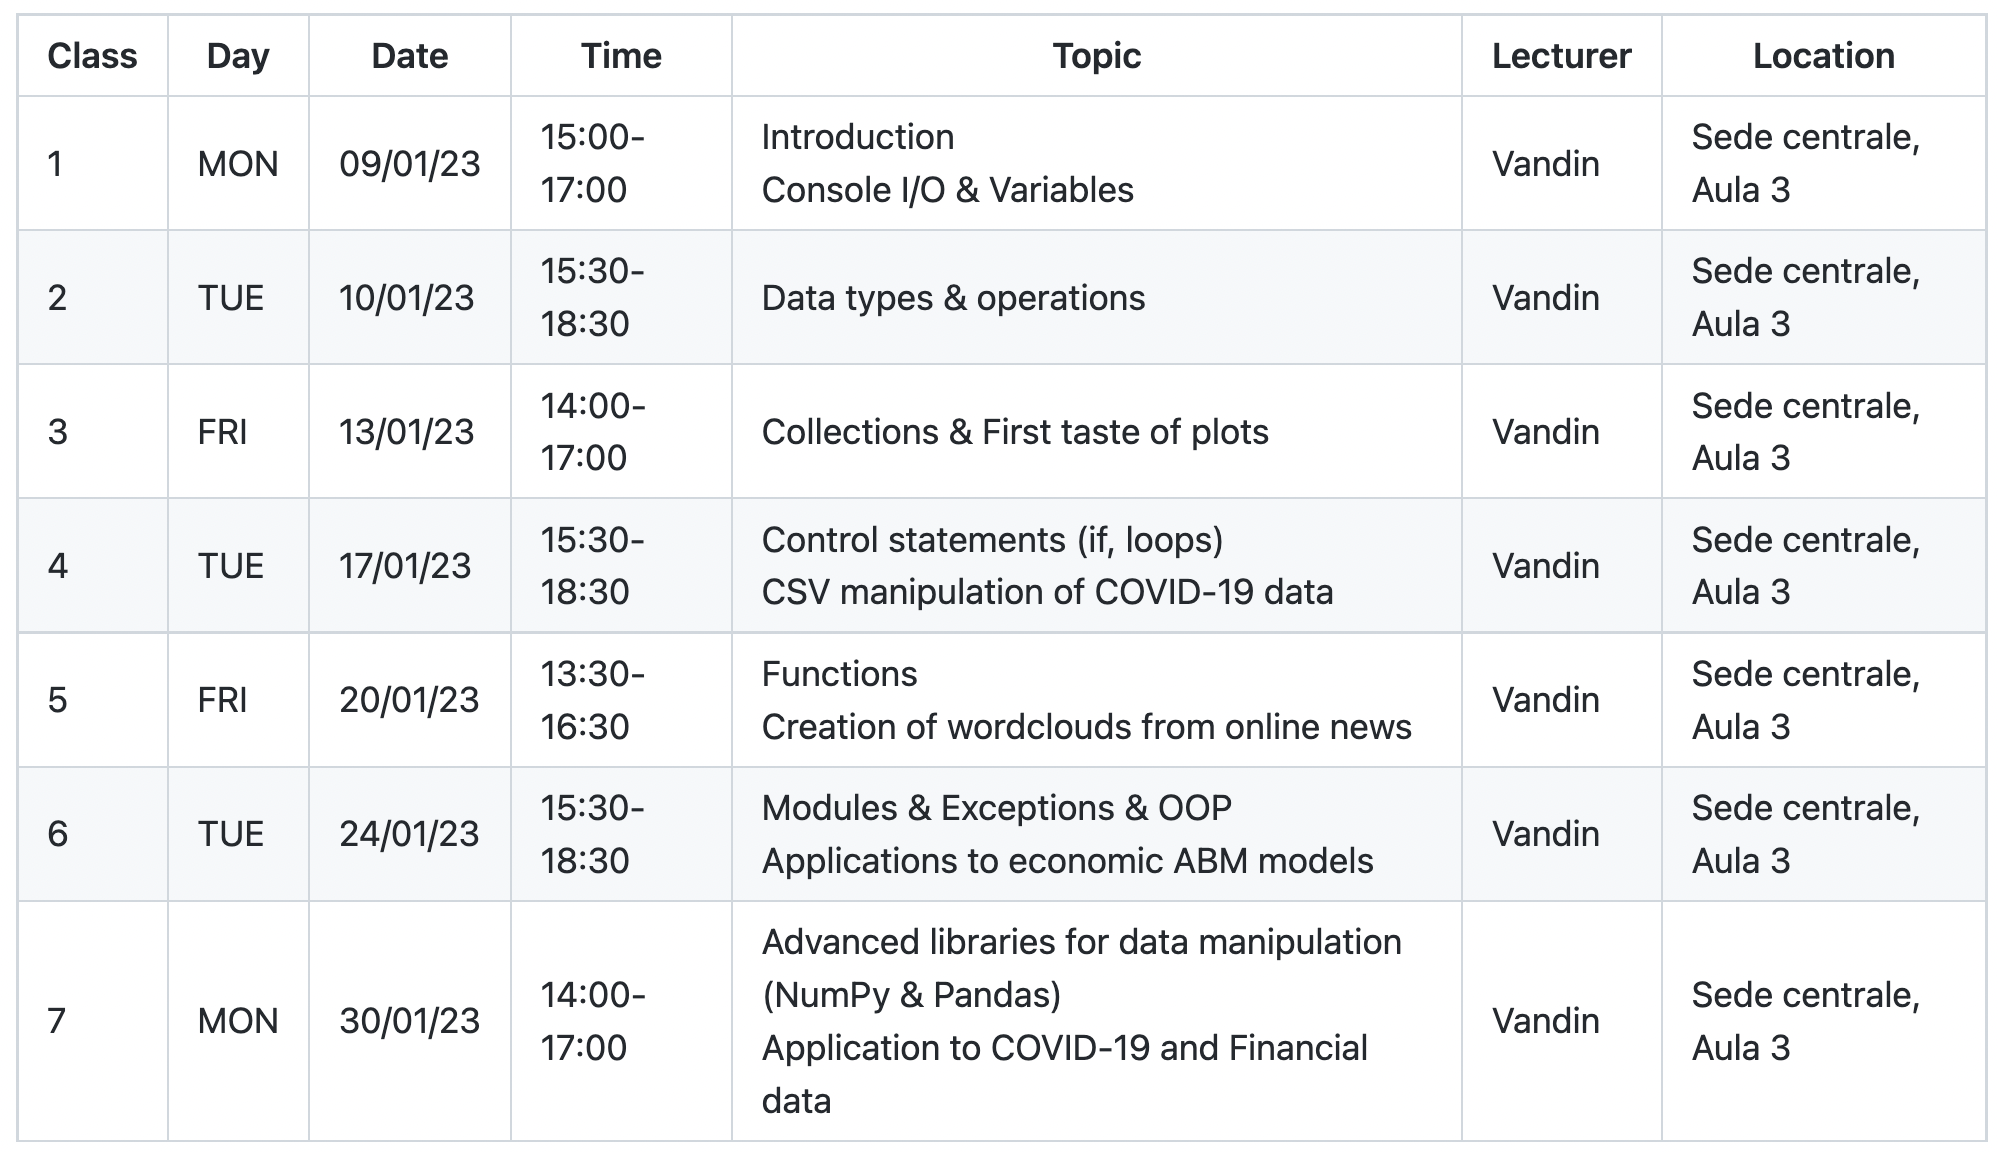
\includegraphics[width=\linewidth]{figures/calendarPDAI1.png}
\end{figure}


%\newcolumntype{H}{>{\setbox0=\hbox\bgroup}c<{\egroup}@{}}
%\scalebox{0.8}{
%  %\ \hspace{-1cm}
%\begin{tabular}{lcc | lH}
%\# & Date & Time & Topic & Chapter \\
%\hline 1 & 14/02 & 15:00-17:00 & Course introduction %\& I/O Console \& Variables 
%& \\
%\hline 2 & 16/02 & 15:00-18:00 & Data types \& operations 
%& \\
%\hline 3 & 18/02 & 15:00-18:00 & Collections %Lists, etc
% & \\
%\hline 4 & 21/02 & 15:00-18:00 & Control and Repetition statements 
%%structures %If \& For 
%& \\
%\hline 5 & 25/02 & 15:00-18:00 & Functions %\& Modules 
%& \\
%\hline 6 & 28/02 & 15:00-18:00 & Modules \& 
%Exceptions \& Object Oriented Programming & \\
%\hline 7 & 04/03 & 15:00-18:00 & 
%Advanced libraries for data  manipulation/visualization
%%Basic data  manipulation \& visualization &
% \\
%\hline
%\hline
%       - & TBD   & \multicolumn{1}{c|}{TBD}         & Exam & \\
%%      & 22.8. & Re-Exam & 
%\end{tabular}
%}
%
%%Swap if/for con collezioni!?  
\end{frame}

\begin{frame}
	\frametitle{Computing, Data Analysis \& Modeling @ L'EMbeDS}
	\centering
\begin{figure}
	%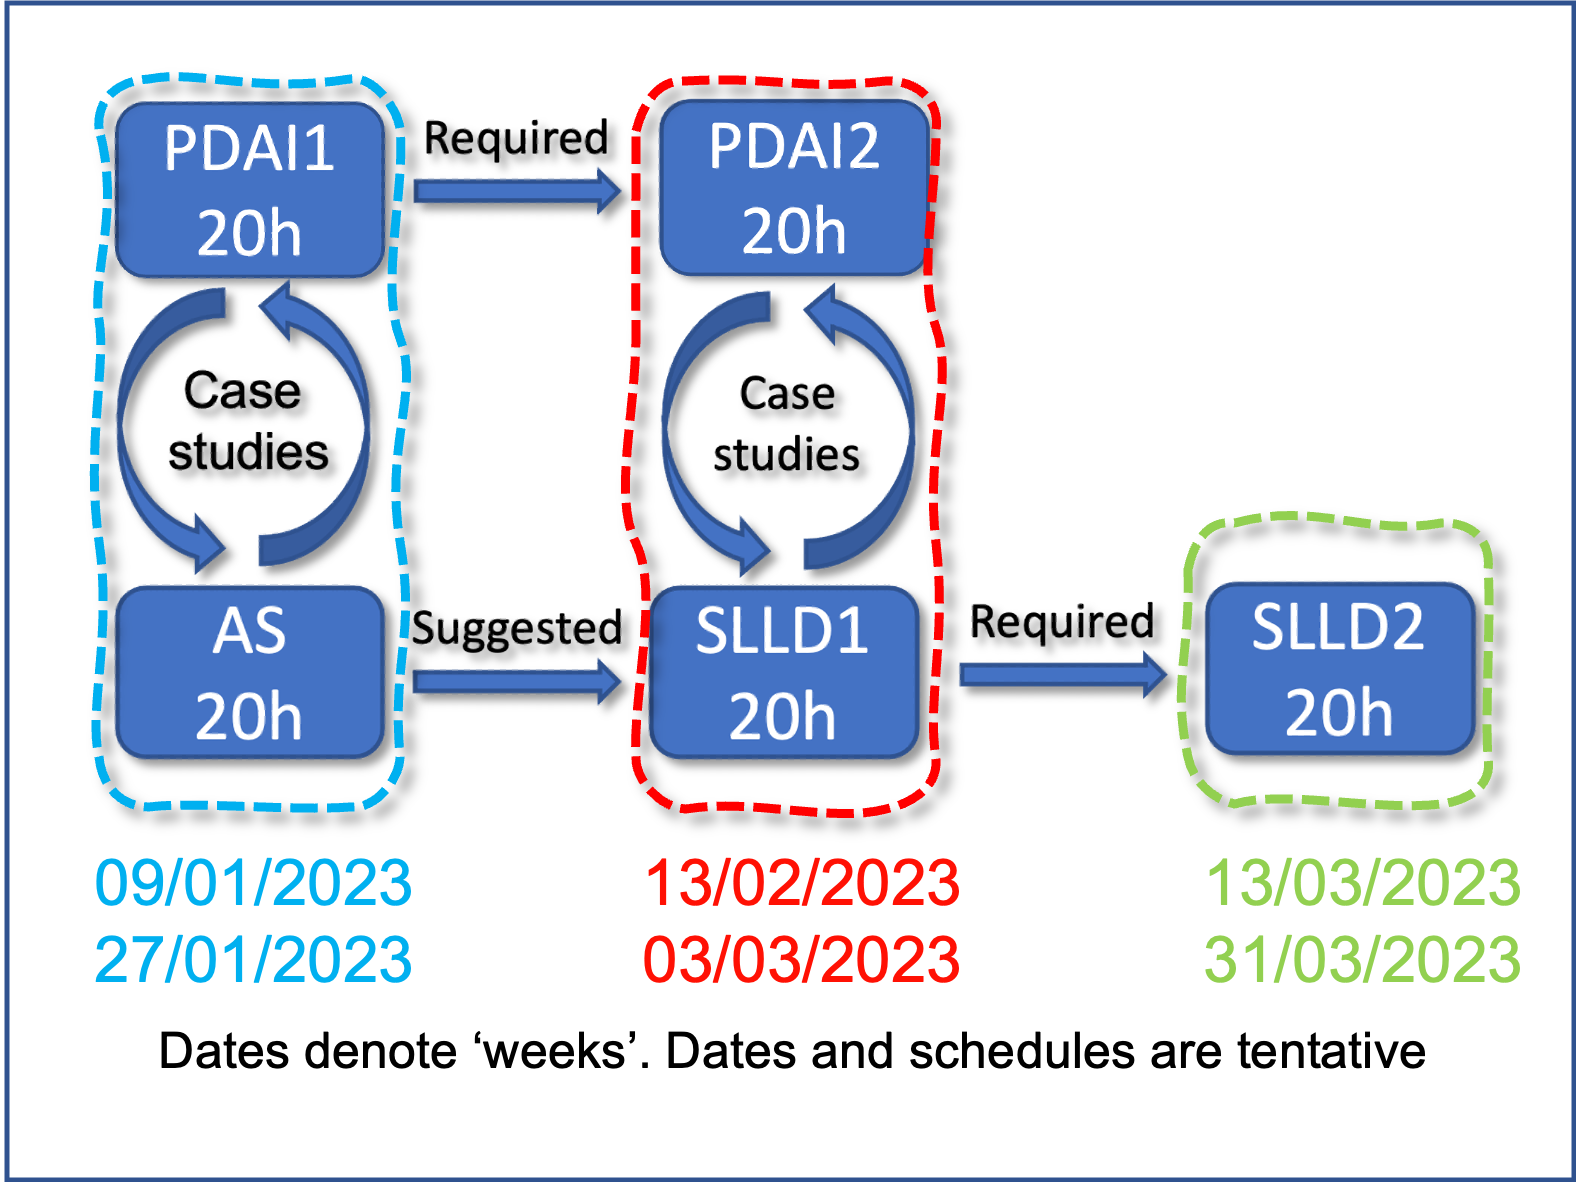
\includegraphics[width=0.95\linewidth]{../../tentativeSchedule.png}
	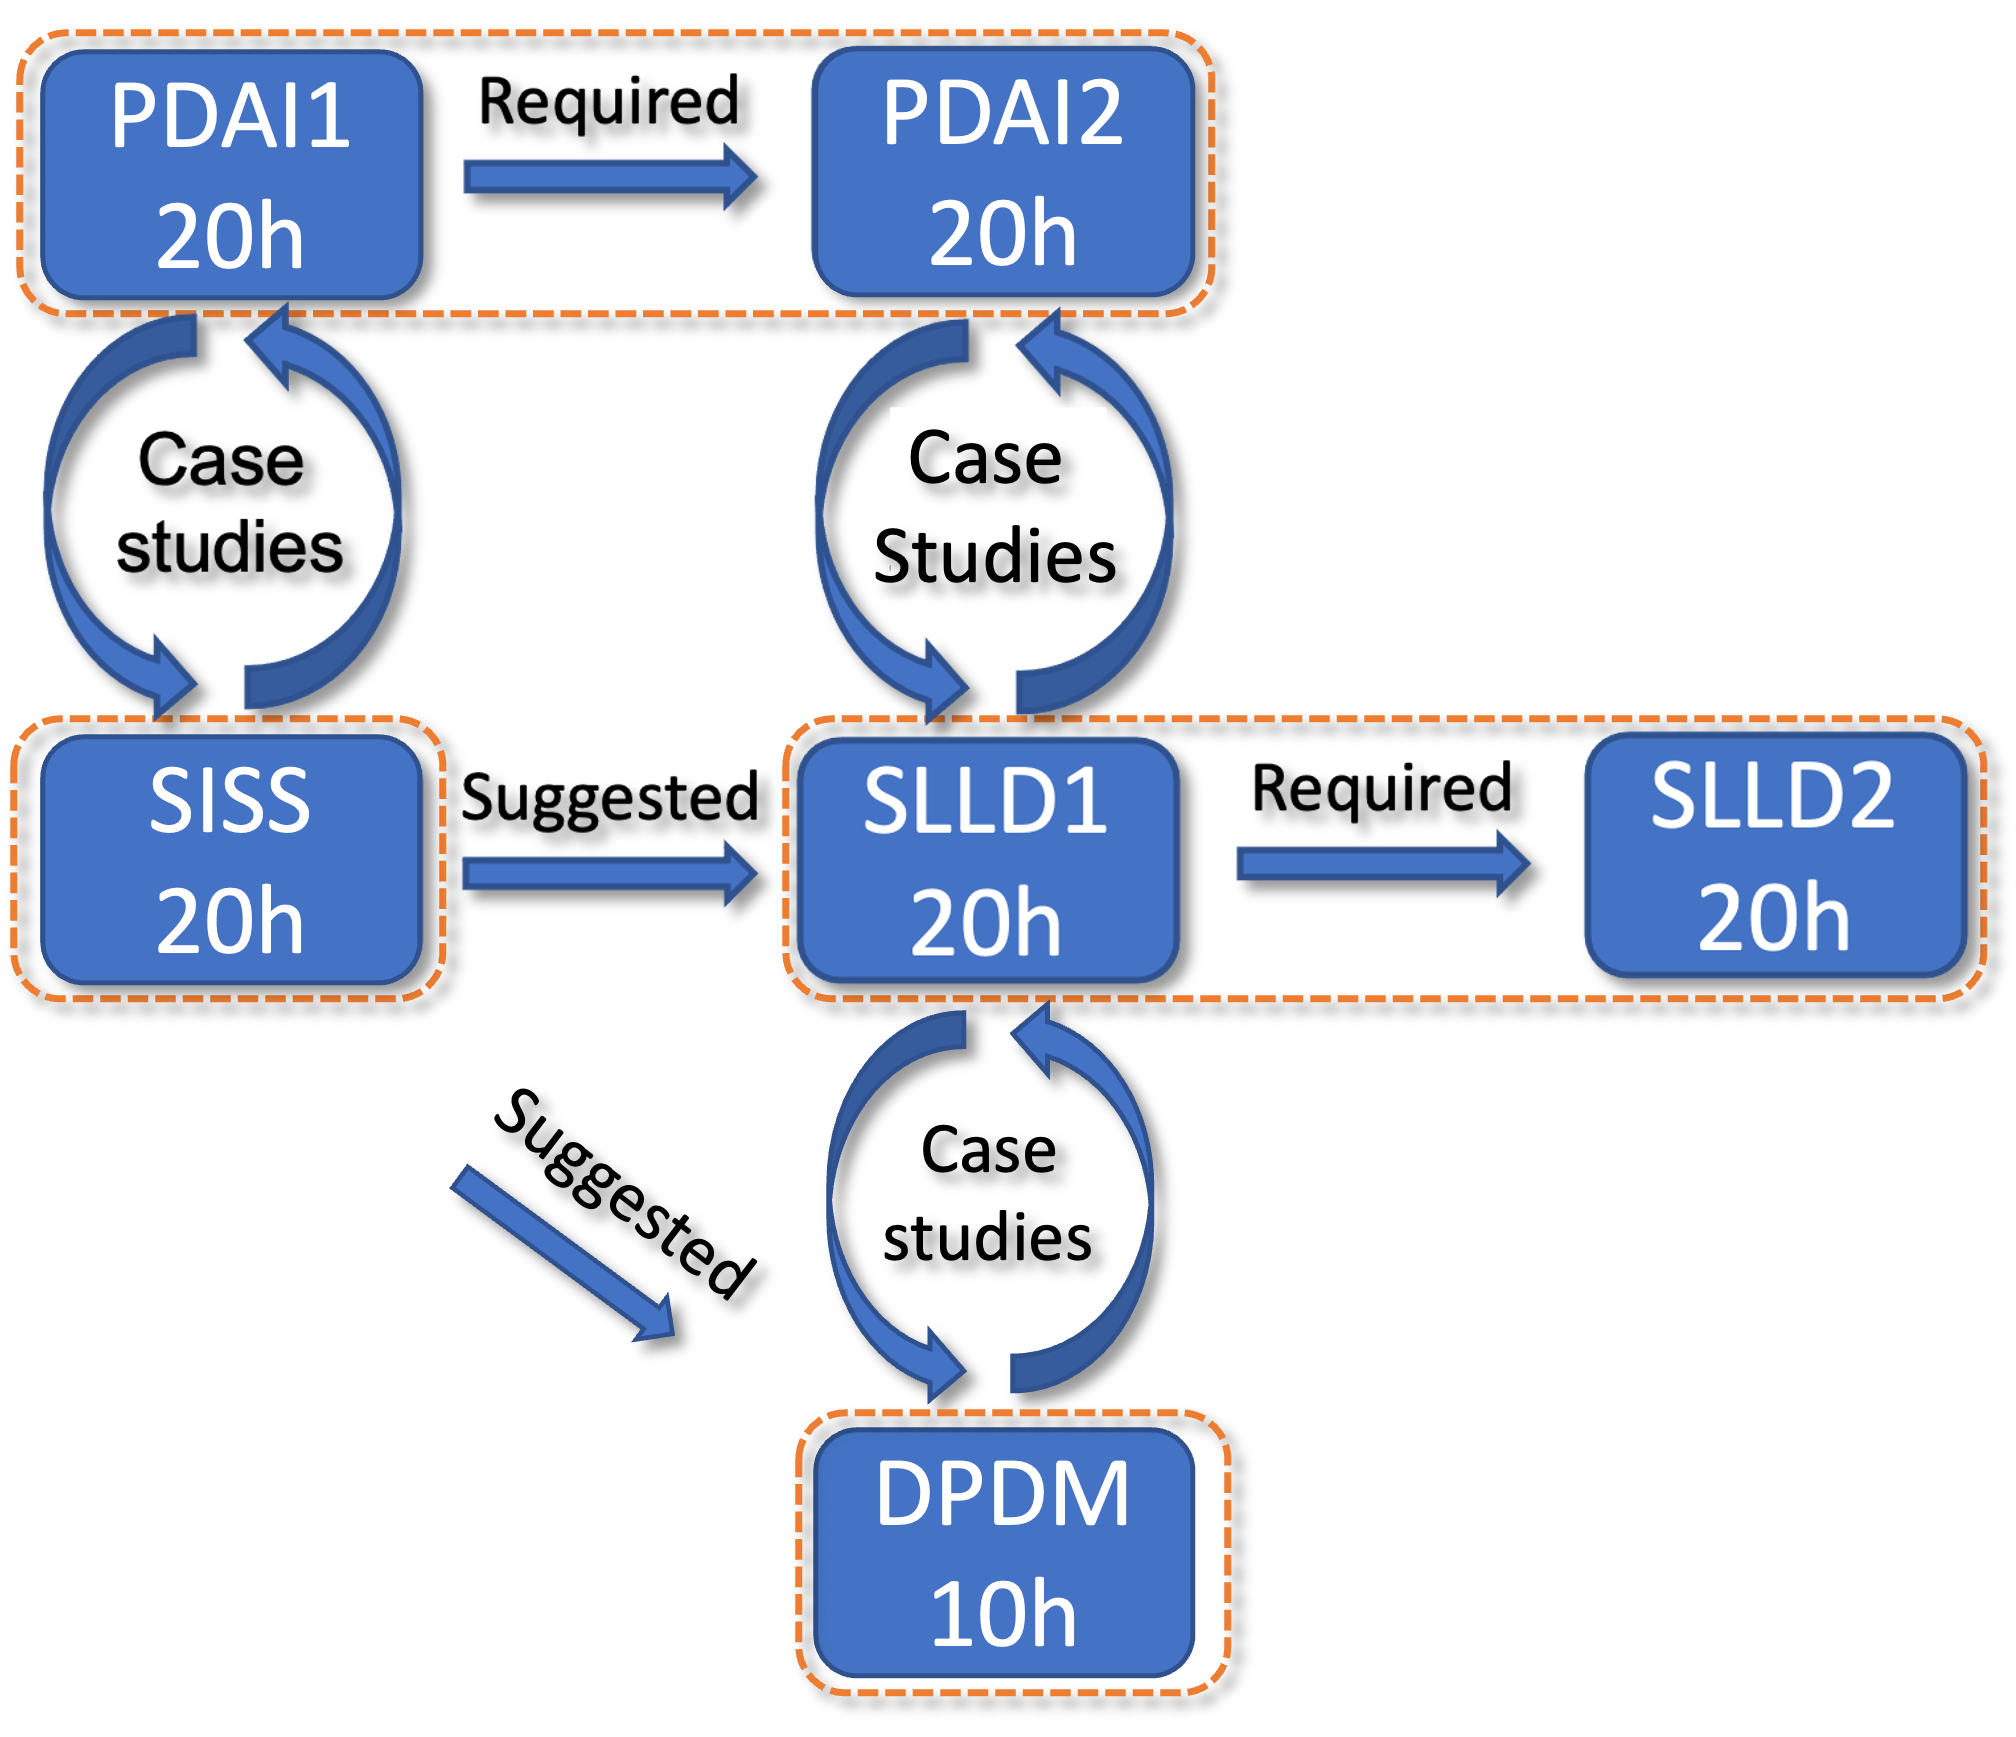
\includegraphics[width=0.8\linewidth]{figures/compDataAnalModel.png}
\end{figure} 
\end{frame}



%\begin{frame}
%  \frametitle{Course Materials}
%  
%\begin{itemize}
%\item Suggested book: M. Lutz, Learning Python.
%\item Software
%\begin{itemize}
%\item Python: \myurl{https://www.python.org/}
%\item Suggested Python editor: JupyterLab \myurl{https://jupyter.org/} 
%%    \begin{itemize}
%%    %\item PyCharm %\myurl{https://www.jetbrains.com/pycharm/}
%%	\item JupyterLab \myurl{https://jupyter.org/} 
%%    \end{itemize}
% \end{itemize}
%\item Setup your machine: 
% \myurl{bit.ly/Intro2Python1920SSSA-setup}
% \end{itemize}
%\end{frame}


\begin{frame}
\frametitle{Further info}
\begin{itemize}
\item No previous experience on computer programming required
\item Previous experience in writing small programs is advantageous
%\item We might adjust the course level according to your expertise and feedback
\pause
\item You will never learn  programming if you don't practice it!
\begin{itemize}
\item \color{red}Therefore you have to regularly do all the assignments
\end{itemize}
\end{itemize}
\end{frame}


\begin{frame}{Ideas for an Effective Course} 
\framesubtitle{Live Programming \& Assignments}
We often have blocks of 3 hours.
\begin{itemize}
\item First part: % (about 2 hours): 
\\ Intro to new topics \& Live programming
    \begin{itemize}
    \item No slides
    \item Iinteractive \emph{notebooks} mixing presentation material and code %during the lecture
%    \item We may make small exercises together in the lecture
      \begin{itemize}
      \item Please have your laptop ready! \myurl{\homepagesetup}
	  \item You find code in advance here %\myurl{\homepageslides}
      \end{itemize}
%	\item Test/consolidate your understanding with the assignments
%      \begin{itemize}
%      \item {\red Assignments are a fundamental learning tool for this course!}
%      \end{itemize}
    \end{itemize}


\item Second part: % (about 1 hour):
\\ You consolidate your understanding working on the assignments
\begin{itemize}
\item Begin working on the assignments with our support if needed
\item Complete them offline before next class. Contact us if needed
\end{itemize}
\end{itemize}
\pause
{\color{red}
However, we have the ambitious goal of covering many topics necessary to introduce you to programming and data analytics in just 20 hours. Hence we might skip some second parts.
}
\end{frame}



\begin{frame}{Live Programming}
\framesubtitle{Find the JupyterLab notebooks at \myurl{\homepageslides}}
\centering 
%\includegraphics[width=0.80\textwidth]{figs/live}
%\includegraphics[width=0.50\textwidth]{figs/liveCrop}
%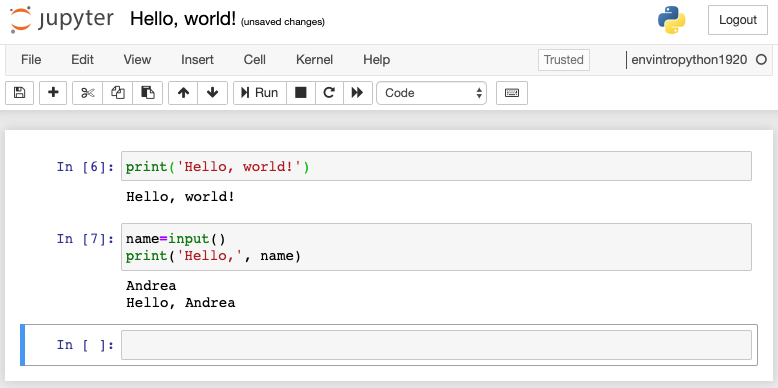
\includegraphics[width=1.0\textwidth]{figures/helloWorld}
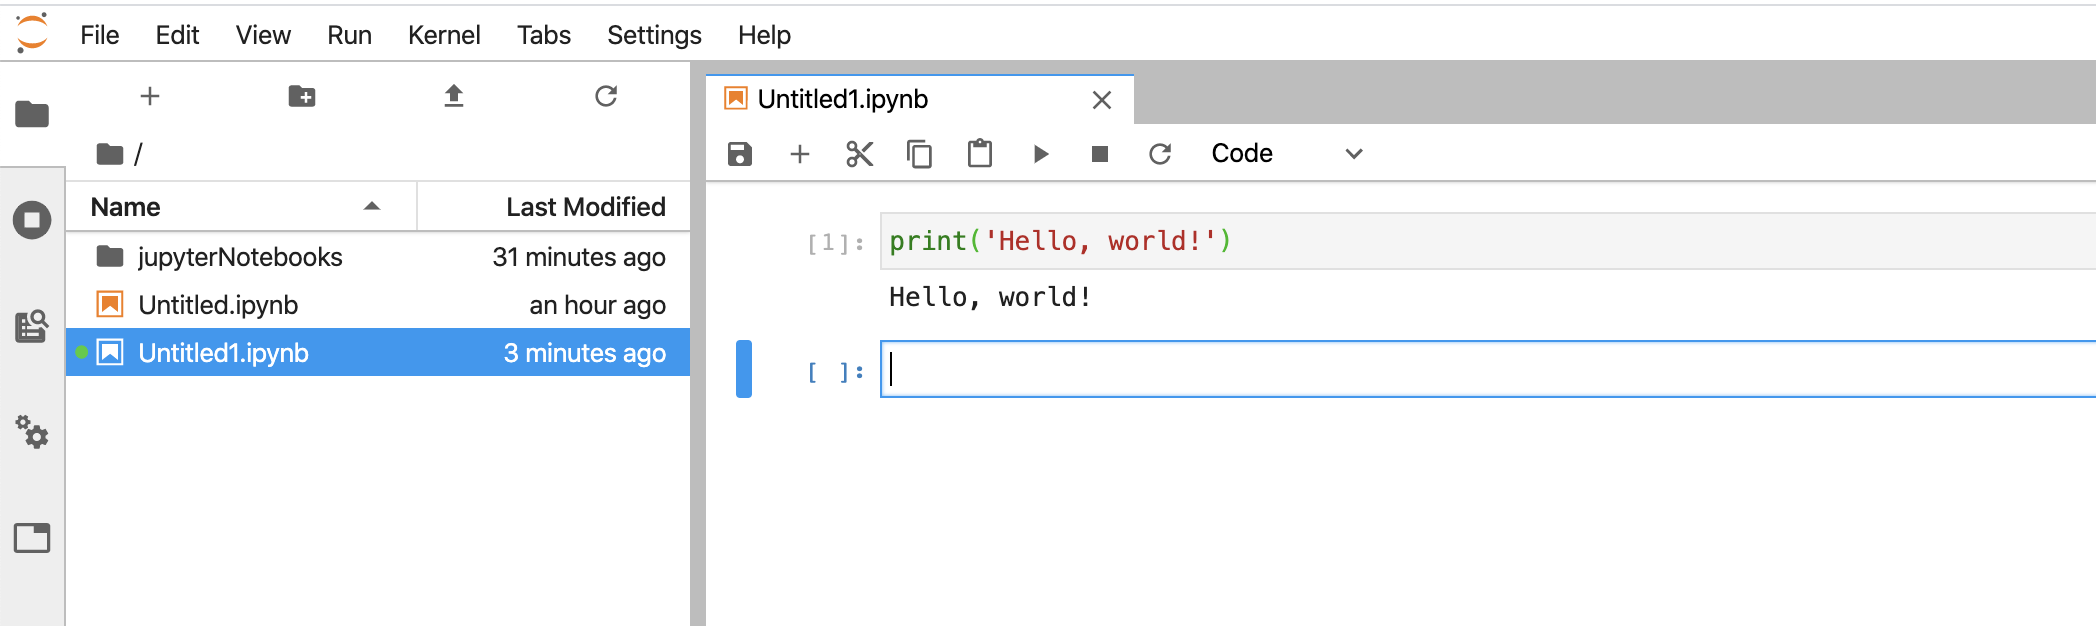
\includegraphics[width=1.0\textwidth]{figures/HelloWorldjupyterlab}
\end{frame}

%\begin{frame}{Live Programming}
%\centering 
%%\includegraphics[width=0.80\textwidth]{figs/live}
%%\includegraphics[width=0.50\textwidth]{figs/liveCrop}
%%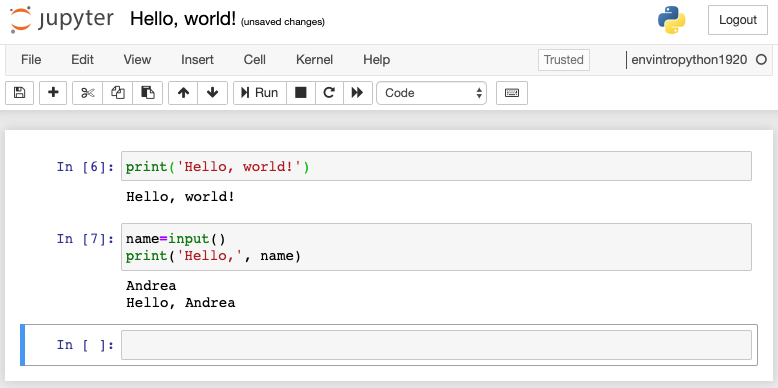
\includegraphics[width=1.0\textwidth]{figures/helloWorld}
%%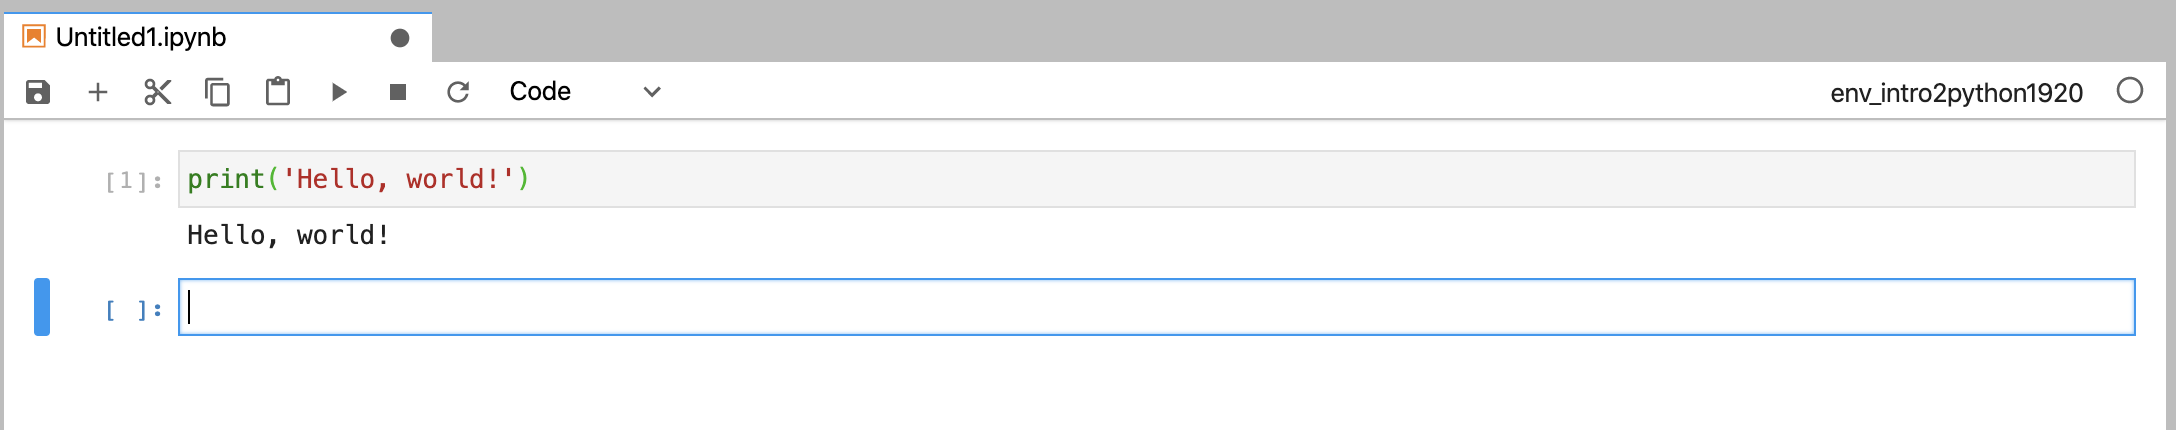
\includegraphics[width=1.0\textwidth]{figures/HelloWorldAfter}
%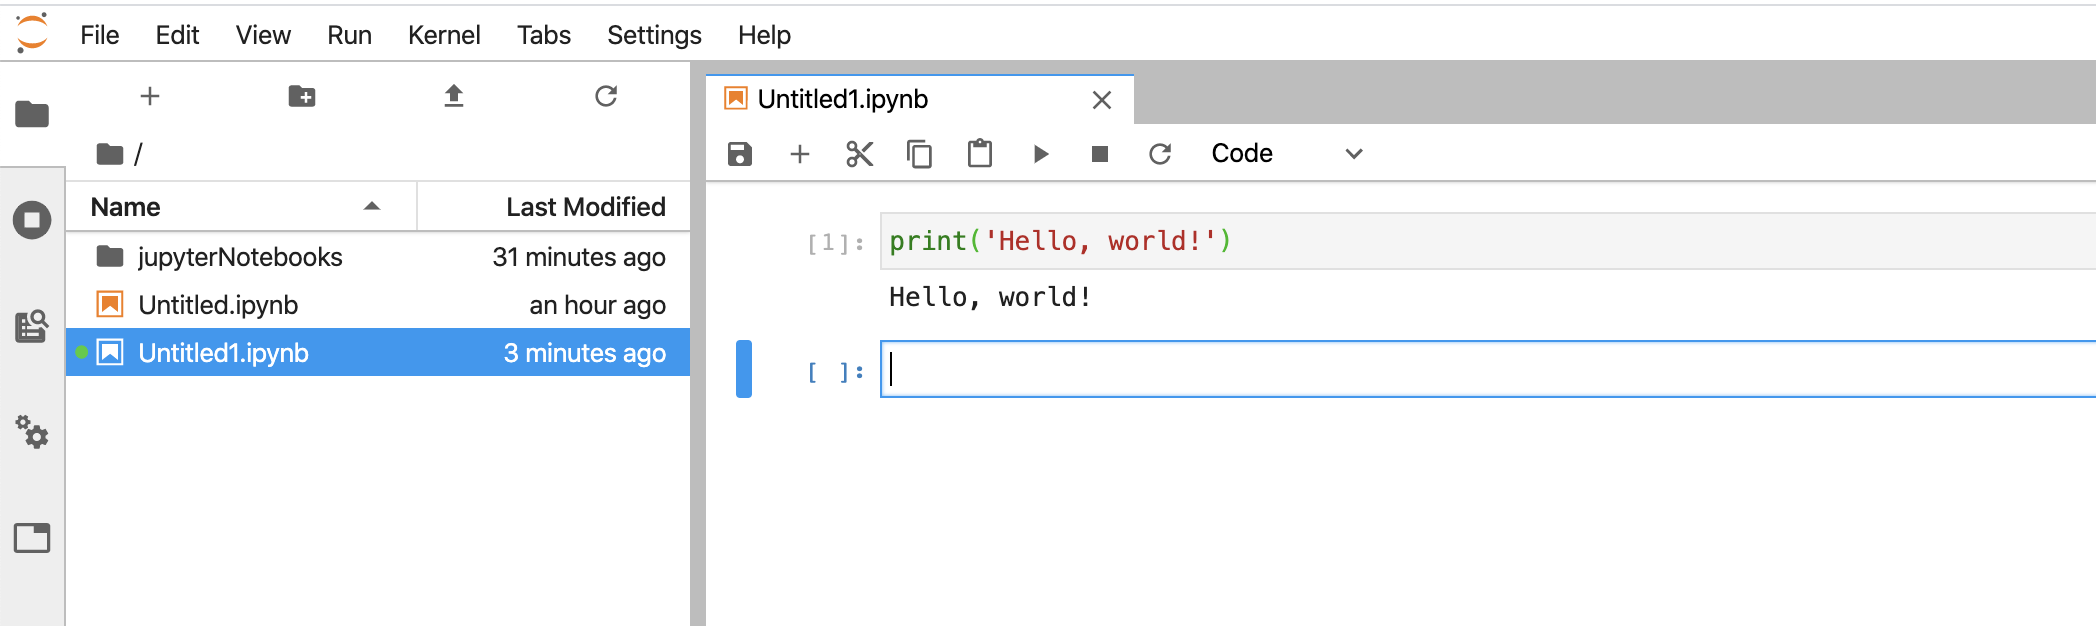
\includegraphics[width=1.0\textwidth]{figures/HelloWorldjupyterlab}
%\end{frame}

%\begin{frame}{Ideas for an Effective Course: CodeJudge}
%  \begin{itemize}
%  \item Exercises using \textit{CodeJudge}
%    \begin{itemize}
%    \item One needs to practice!
%    \item Immediate feedback from \textit{CodeJudge} which tests your code
%%    \item Demo and first exercises next week
%    \end{itemize}
%  \end{itemize}
%\end{frame}

%\begin{frame}{Repl.it}
%\centering 
%% 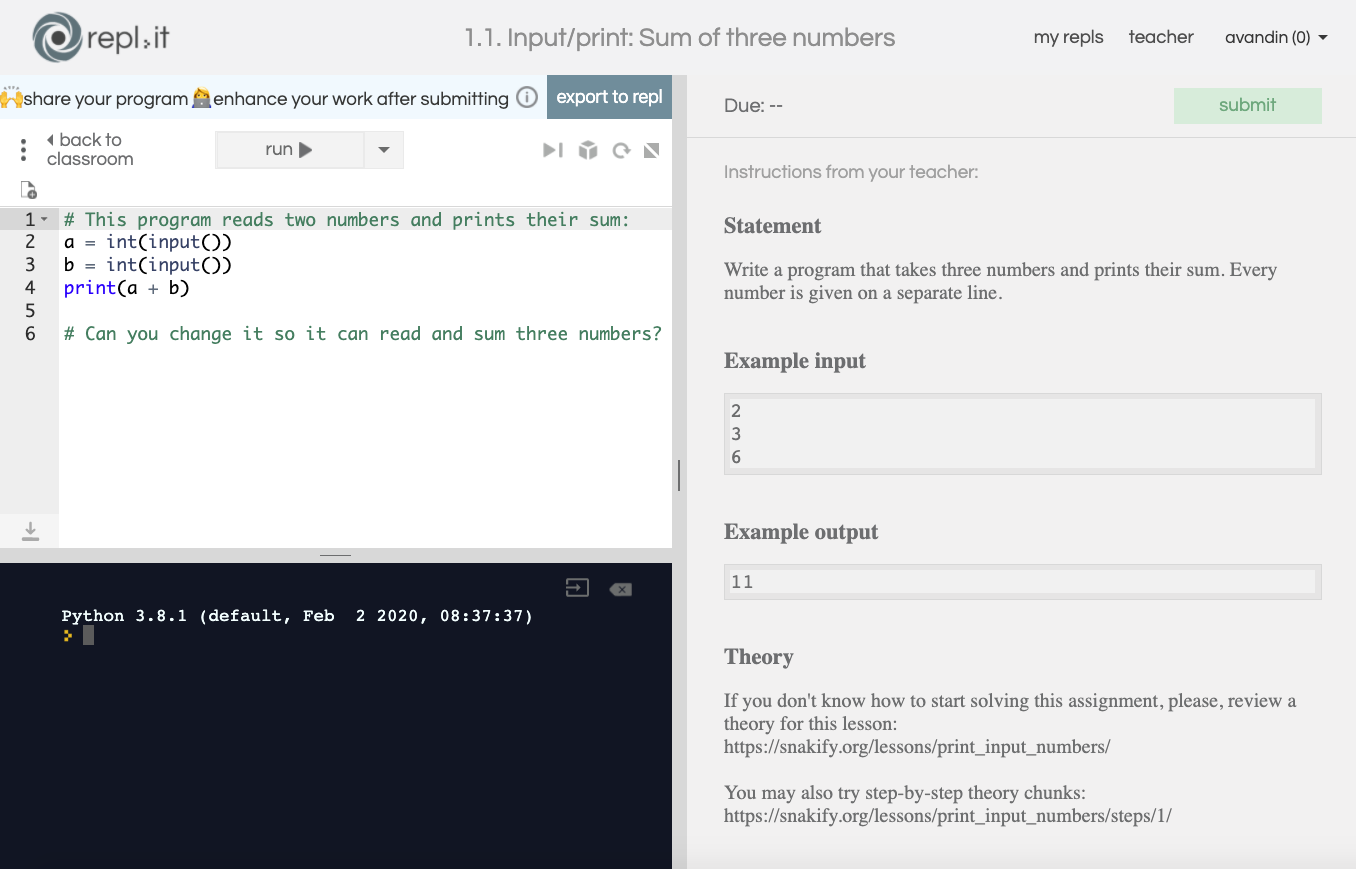
\includegraphics[width=0.9\textwidth]{figures/repl}
% 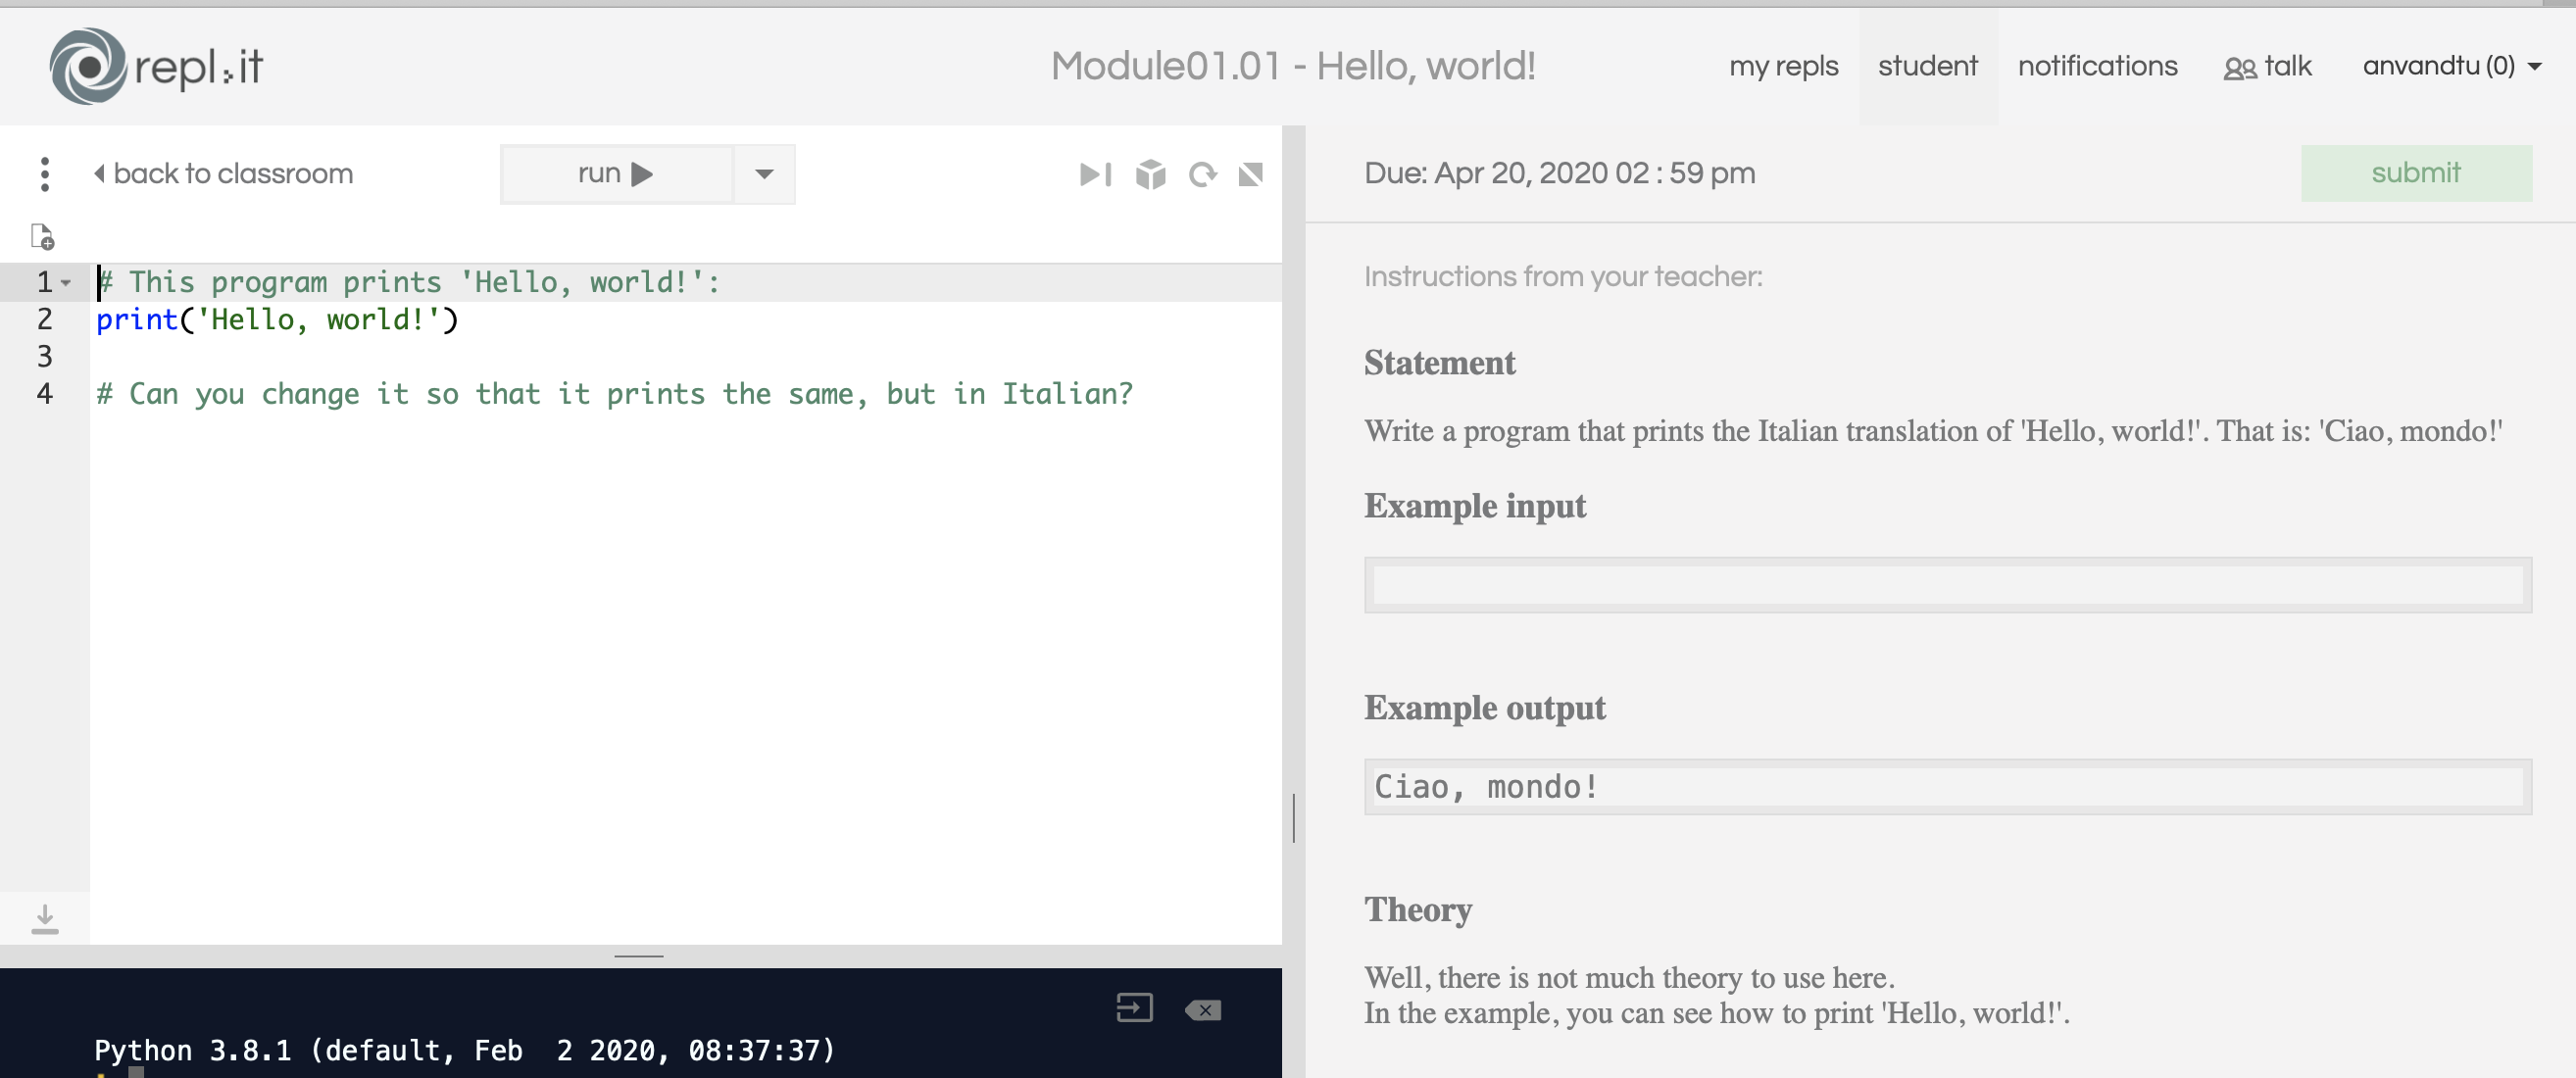
\includegraphics[width=1.0\textwidth]{figures/replNew}
%\begin{itemize}
%\item First time visit:
%\myurl{\replstudentsinvitation}
%\item After that: \hspace{0.58cm} \myurl{\replstudents}
%\end{itemize}
%\end{frame}
%
%\begin{frame}{Repl.it}
%\centering 
%\begin{itemize}
%\item A Repl.it team is a collection of assignments with autograding functionalities
%\item Your dashboard will be an ordered list of assignments. \\ You can see the status of your assignments
%\item Our dashboard tells us the status of all your assignments
%\end{itemize}
%\end{frame}

\begin{frame}{Assignments on Colab}
	\centering 
	% 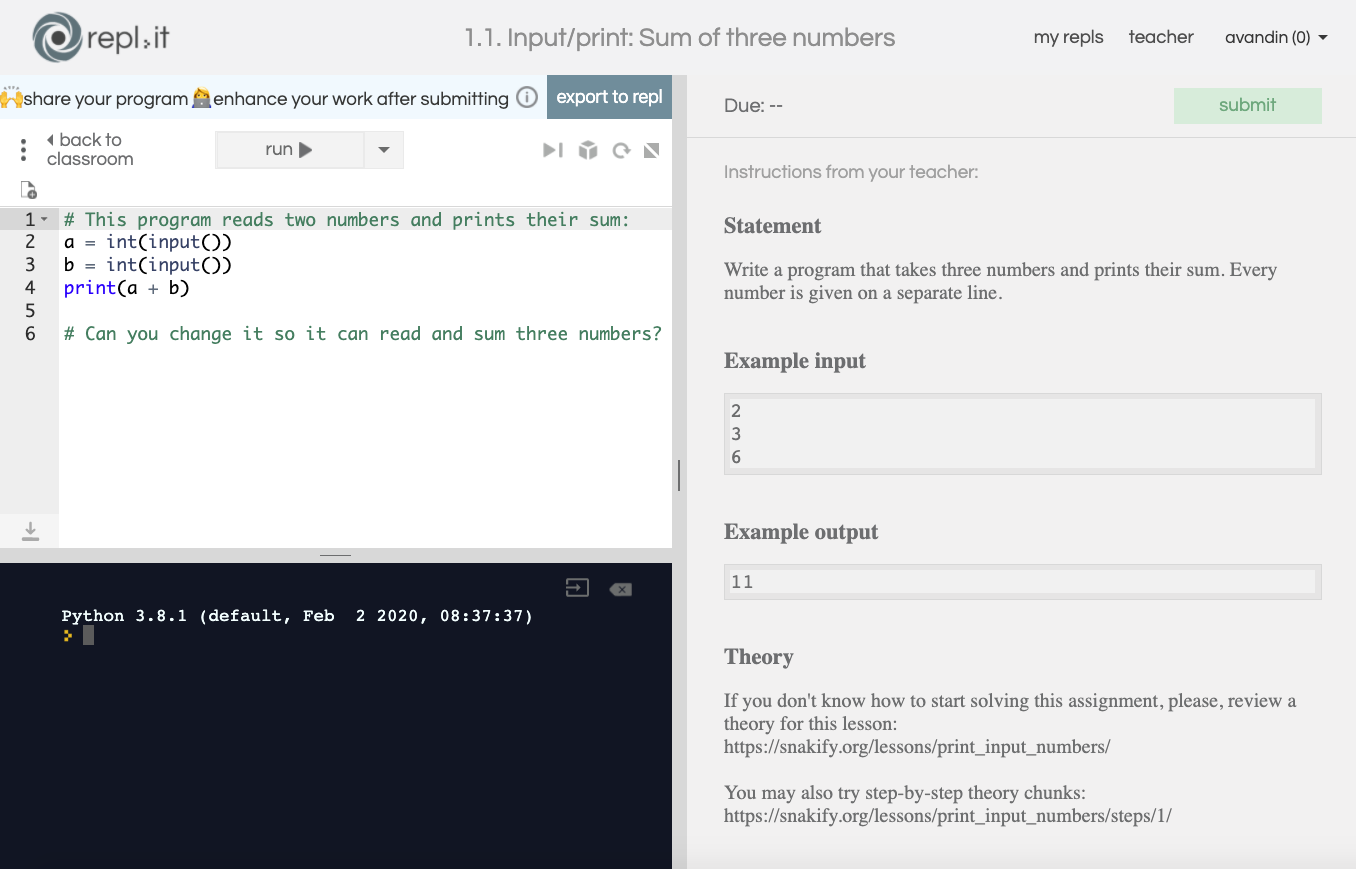
\includegraphics[width=0.9\textwidth]{figures/repl}
	% 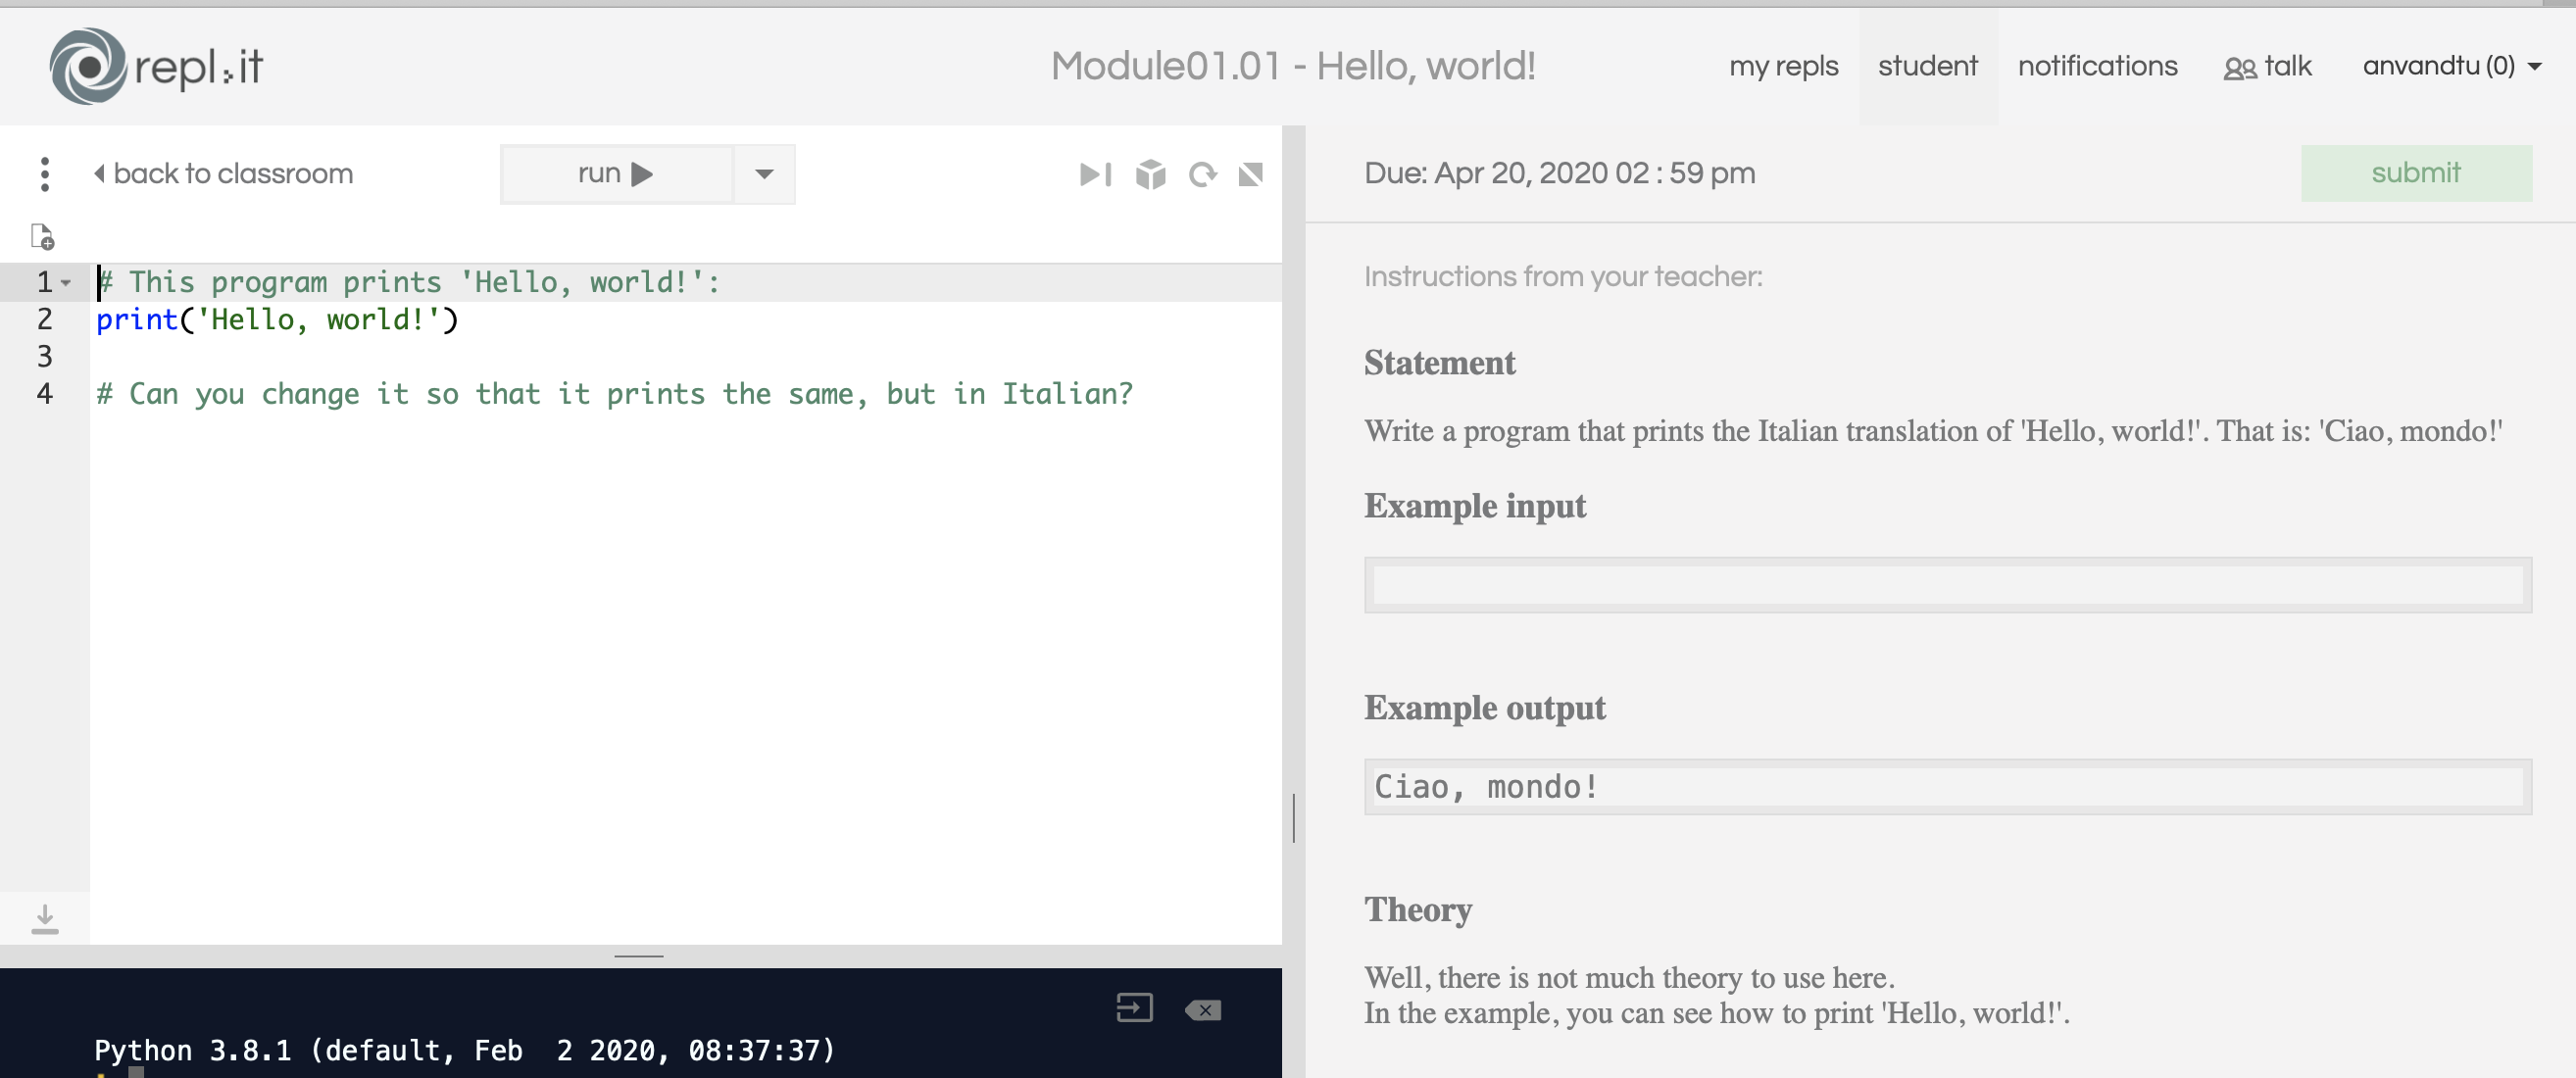
\includegraphics[width=1.0\textwidth]{figures/replNew}
	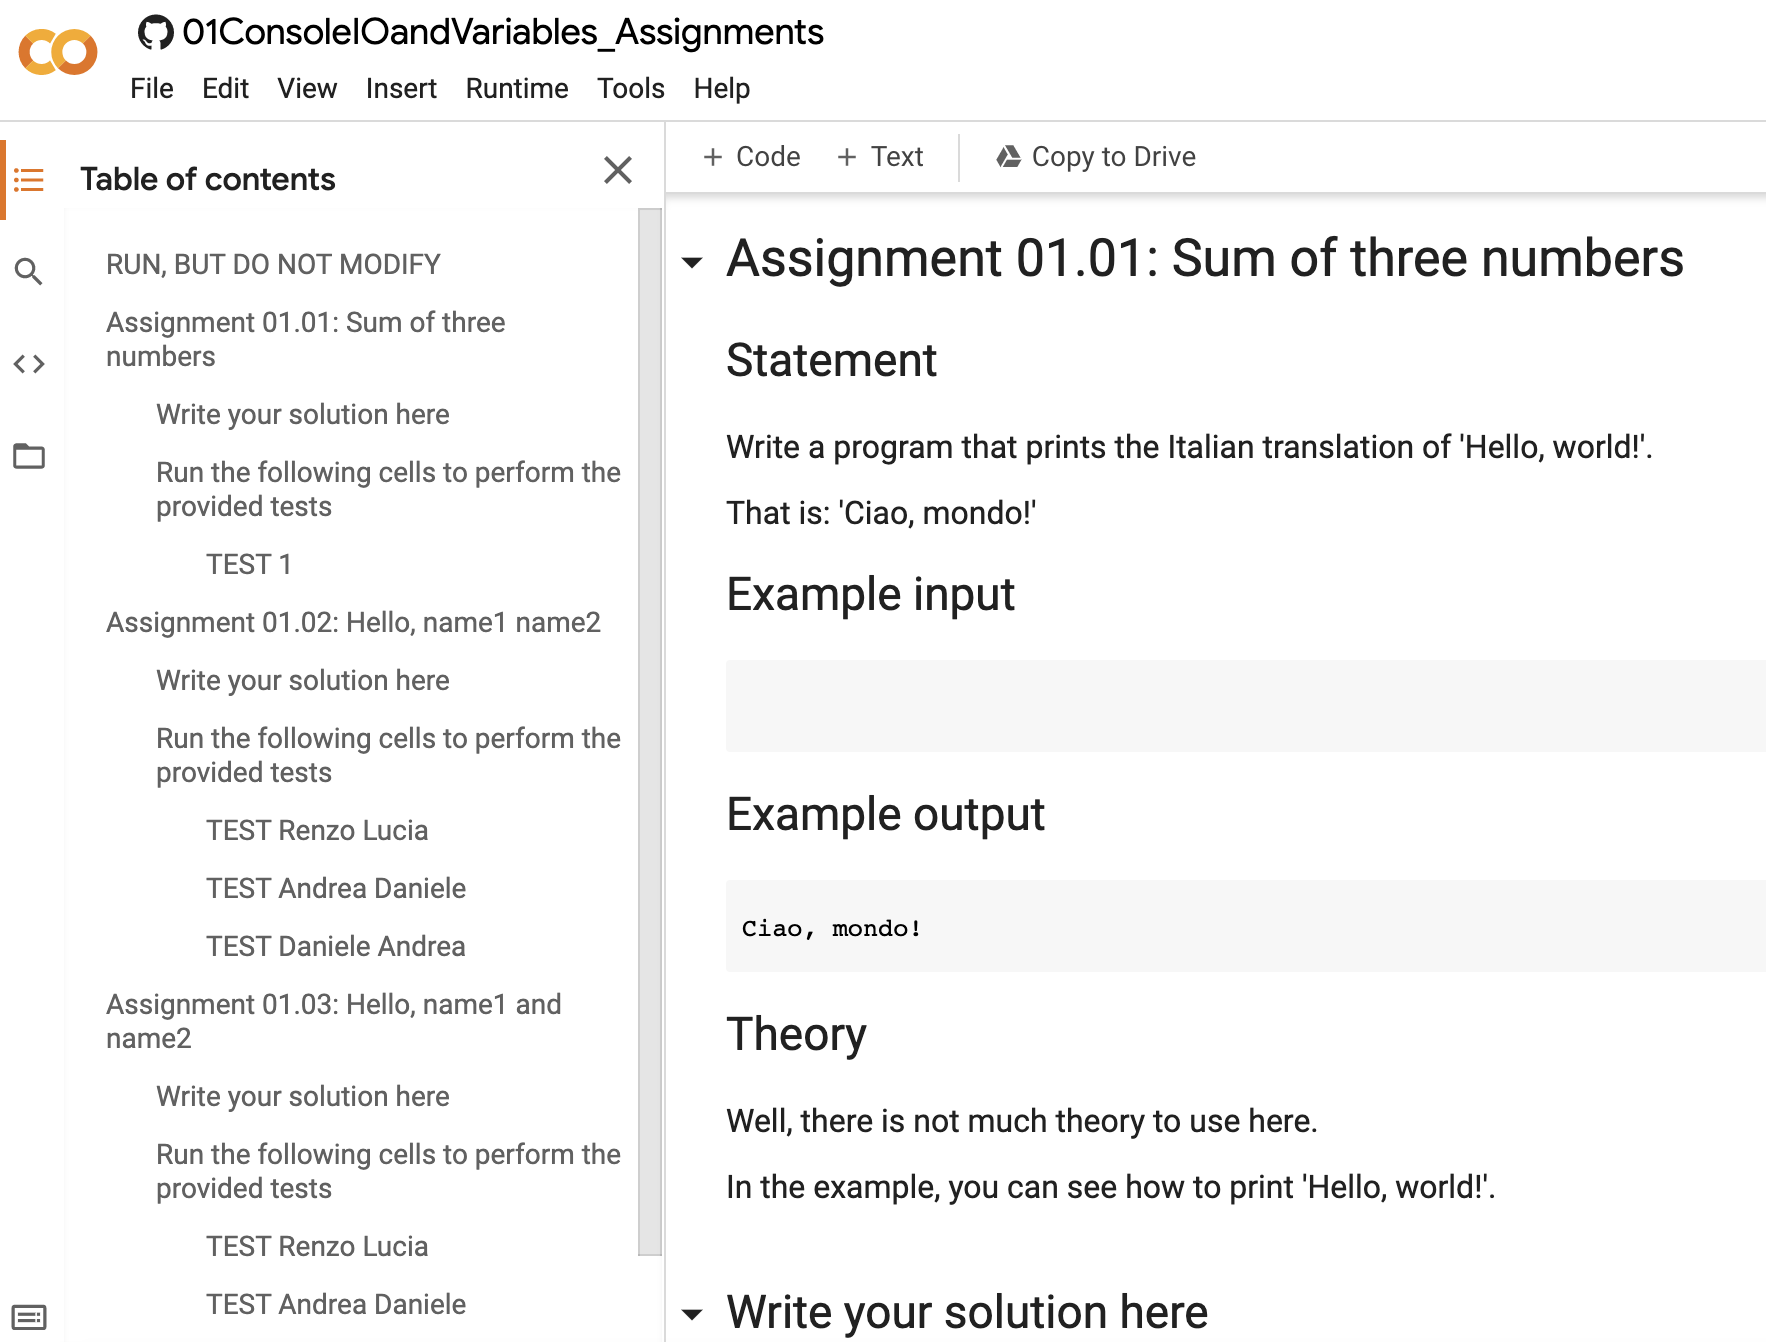
\includegraphics[width=0.78\textwidth]{figures/colab1}
	\begin{itemize}
		\item Each lecture comes with a set of simple coding assignments
		\begin{itemize}
			%\item Distributed using Colab
			\item Links available in the wiki page for slides and further material
		\end{itemize}
	\end{itemize}
\end{frame}

\begin{frame}{Colab}
	\centering 
	\begin{itemize}
		\item Colab is a Google service similar to Google docs 
		\begin{itemize}
			\item but for python notebooks.
			\item no installation required
		\end{itemize}	
		\item Each set of assignments is actually a python notebook
		\item We implemented in Colab autograding functionalities
		\begin{itemize}
			\item to test your solution
		\end{itemize}	
		%\item If you prefer, you can also download them as jupyter notebooks
	\end{itemize}
\end{frame}

\begin{frame}{Colab: auto-testing}
	\centering 
	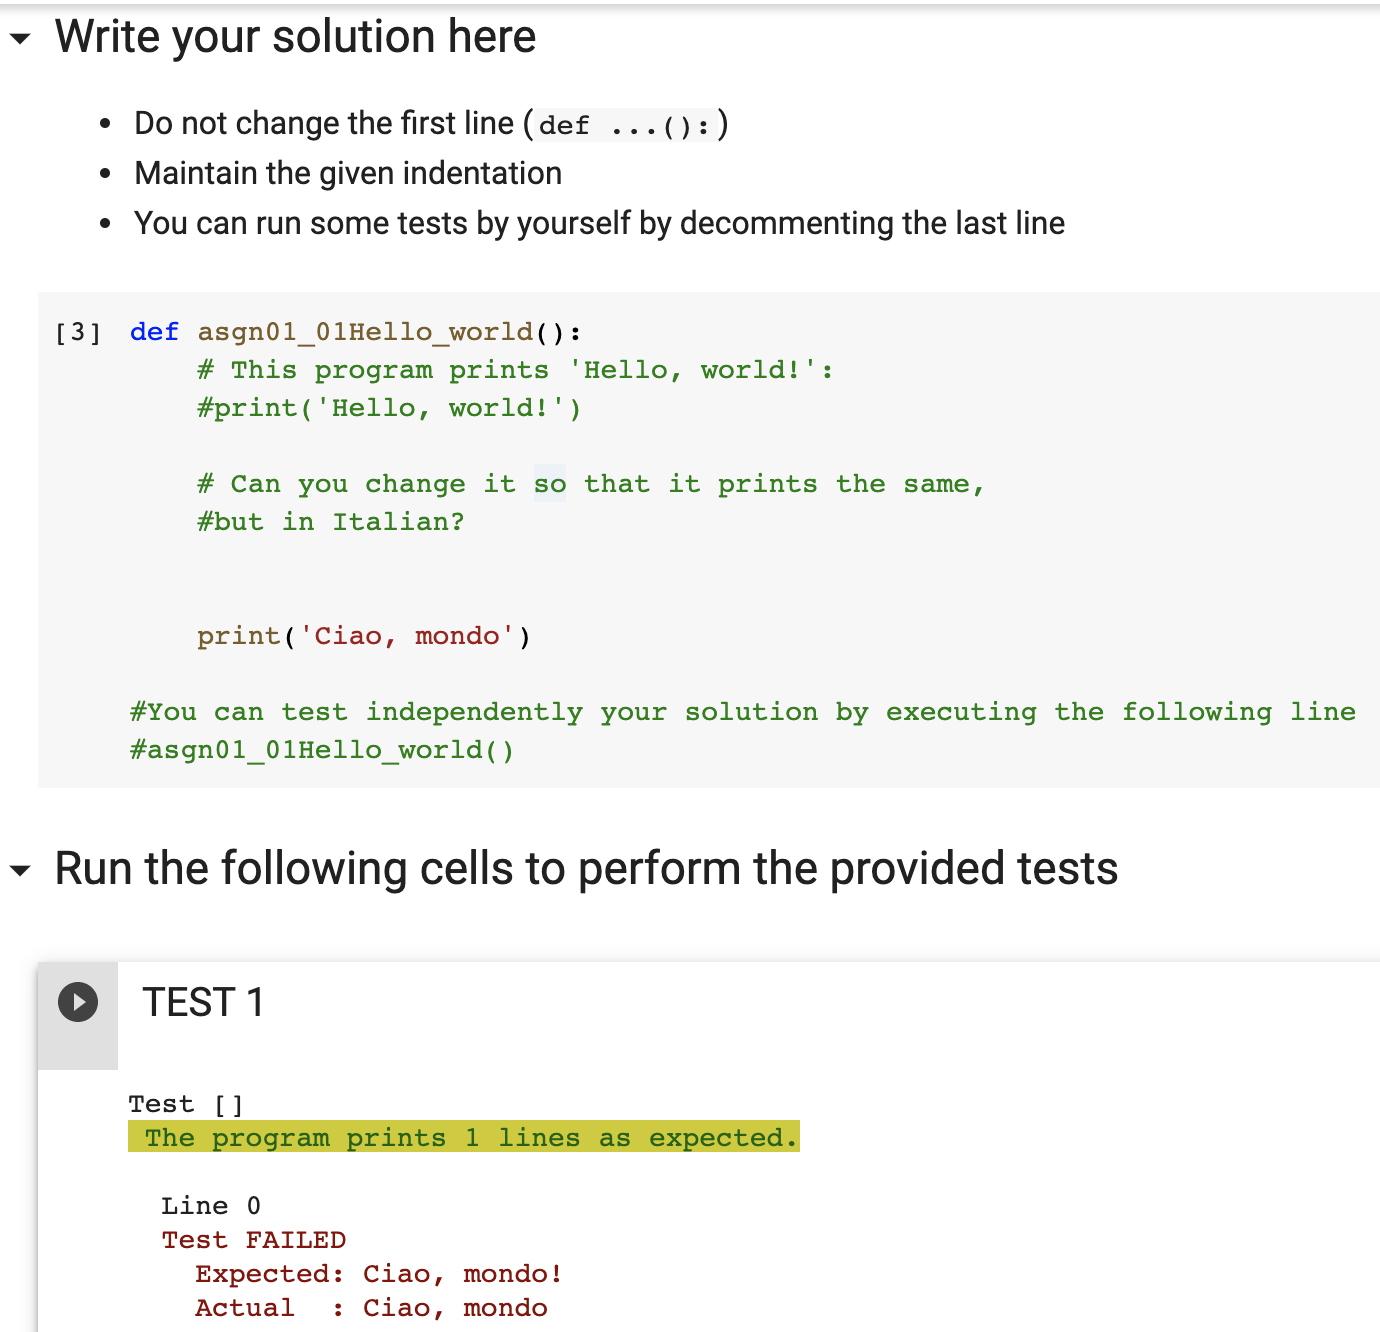
\includegraphics[width=0.67\textwidth]{figures/colab3b}
\end{frame}

\begin{frame}{Colab: auto-testing}
	\centering 
	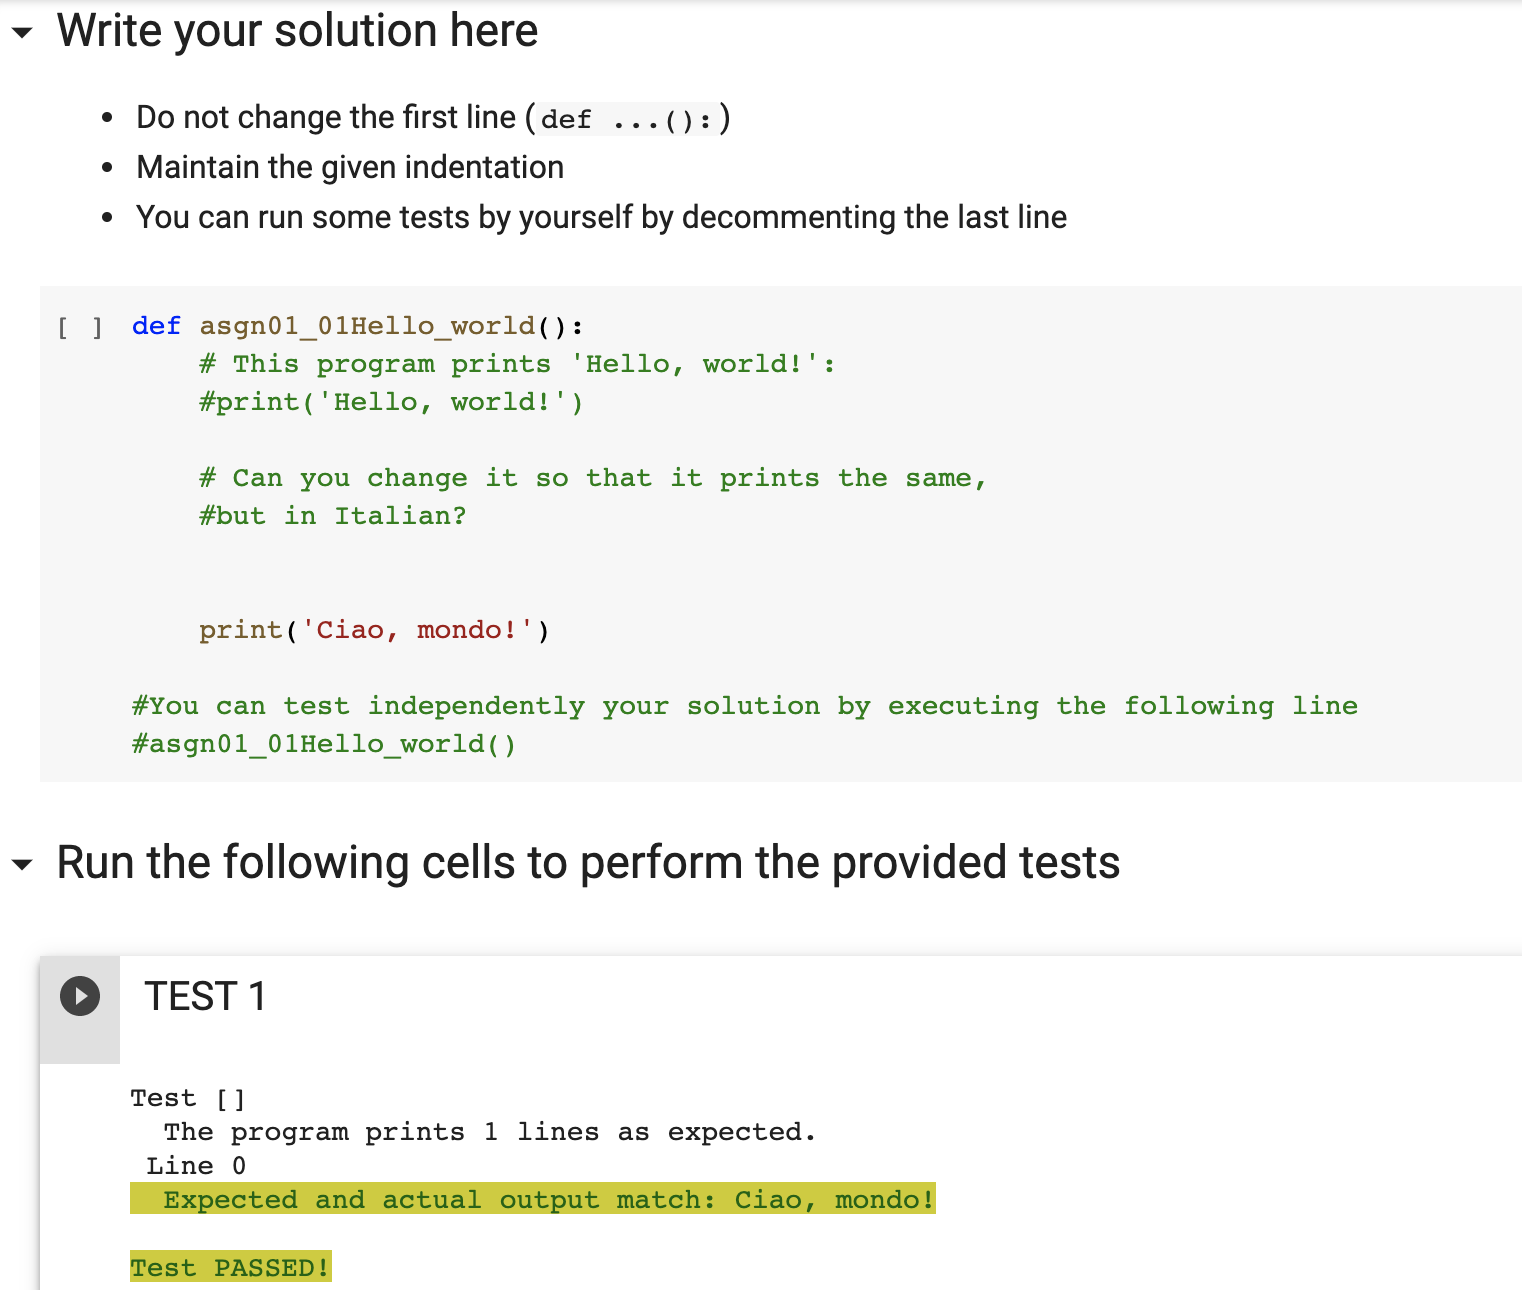
\includegraphics[width=0.72\textwidth]{figures/colab2}
\end{frame}


\section{Sneak preview of Module 2}
\begin{frame}{Outline}
	\tableofcontents[currentsection]
\end{frame}

\begin{frame}{Sneak preview of Module 2}
	\centering 
	Starting from the competences developed in the first module, we will study
	how to apply data analysis techniques from Machine learning
%	
\includegraphics[width=0.4\linewidth]{figures/whats_ml.jpg}
	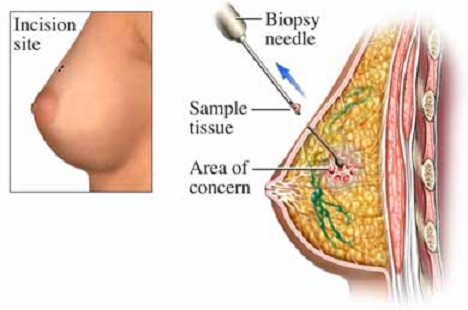
\includegraphics[width=0.4\linewidth]{figures/Breast-Biopsy-2.jpg}\\
	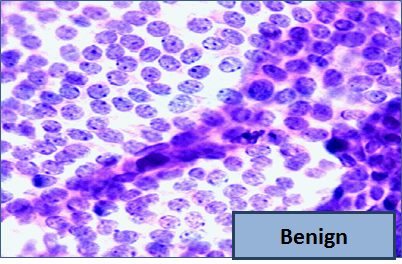
\includegraphics[width=0.4\linewidth]{figures/fna-benign1.png}
	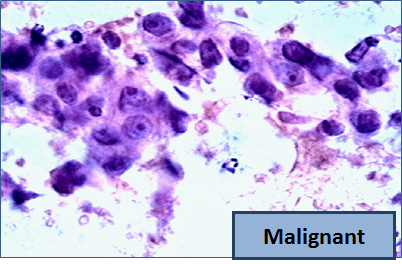
\includegraphics[width=0.4\linewidth]{figures/fna-malignant1.png}\\
	Can we classify them automatically?
\end{frame}

\begin{frame}{Sneak preview of Module 2}
	We will go through a classic pipeline for these data analysis tasks
\begin{itemize}
	\item With emphasis on how to do \emph{good} data analysis projects
	\item We explain how to avoid common pitfalls of \emph{bad} analysis projects
	\end{itemize}		
%We will use two alternative approaches 
%	\begin{itemize}
%		\item Python: \textbf{main focus}
%		\item Knime: a graphical workflow language
%	\end{itemize}		
%\centering
%	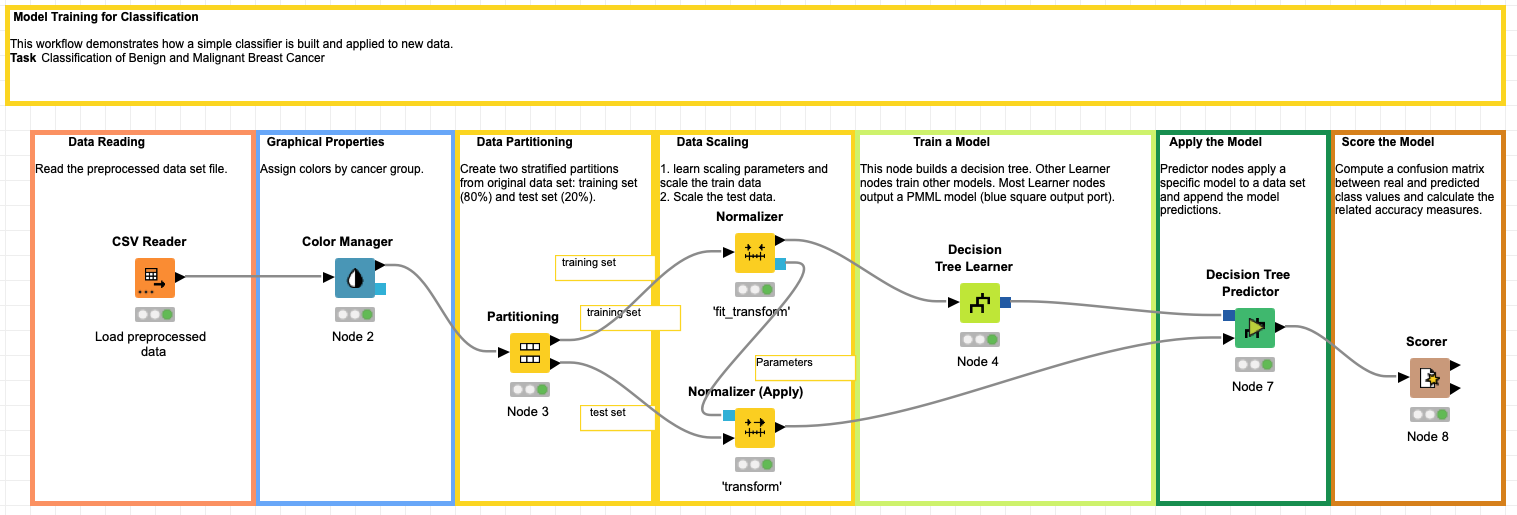
\includegraphics[width=1.0\linewidth]{figures/knimepipeline.png}
\end{frame}

\begin{frame}{Sneak preview of Module 2}
	\centering 
	Further advanced research-oriented topics of data-driven analysis like Process Mining \\
	
	%	
\includegraphics[width=0.4\linewidth]{figures/whats_ml.jpg}
	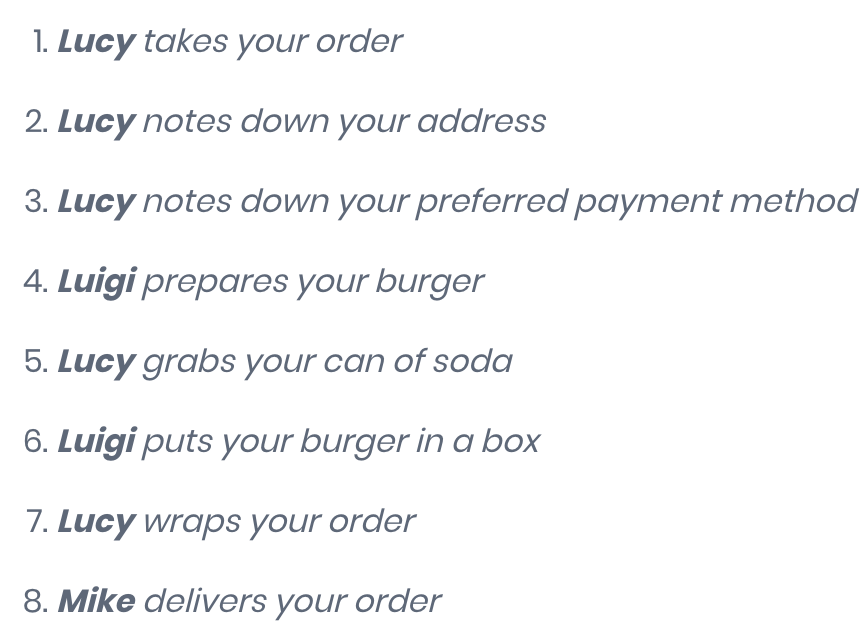
\includegraphics[width=0.4\linewidth]{figures/lucy.png}
	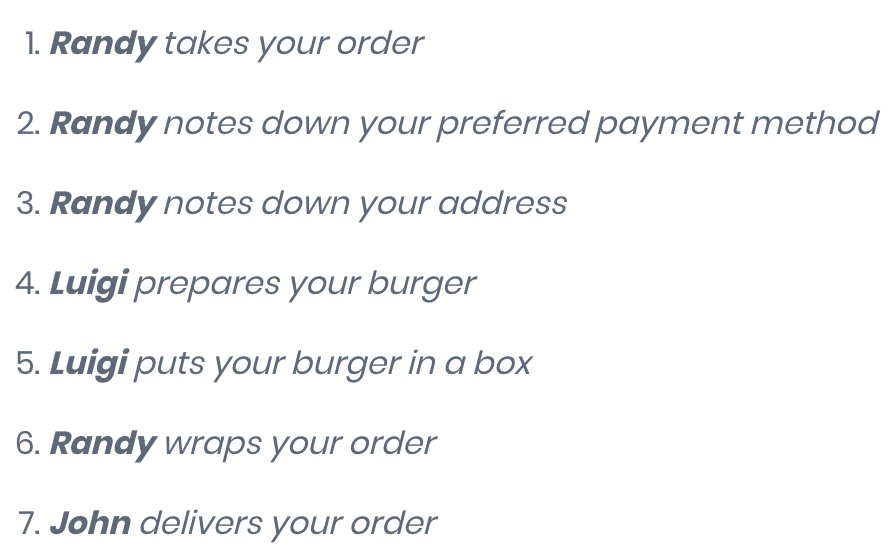
\includegraphics[width=0.4\linewidth]{figures/randy.png}\\
		\textbf{What is the process underlying my data?}\footnote{Example from \url{https://pm4py.fit.fraunhofer.de/}}\\
	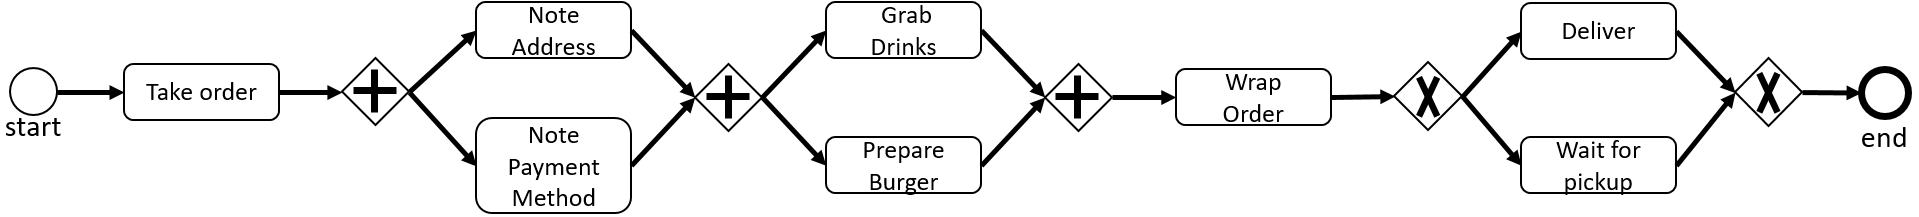
\includegraphics[width=0.9\linewidth]{figures/simple_sample_model.png}
	
\end{frame}

\begin{frame}{Sneak preview of Module 2}
	\begin{block}{Evaluation}
		You will do the same on data of interest or on data on titanic sinking
	\begin{itemize}
		\item Would you have survived the sinking of the titanic?
	\end{itemize}
\begin{itemize}
	\item Alternatively: bring your own data of interest!
\end{itemize}
	\end{block}
	
\end{frame}

\section{Let's Kahoot!}
\begin{frame}{Outline}
	\tableofcontents[currentsection]
\end{frame}

\begin{frame}{Let's play a game on Kahoot!}
	\centering
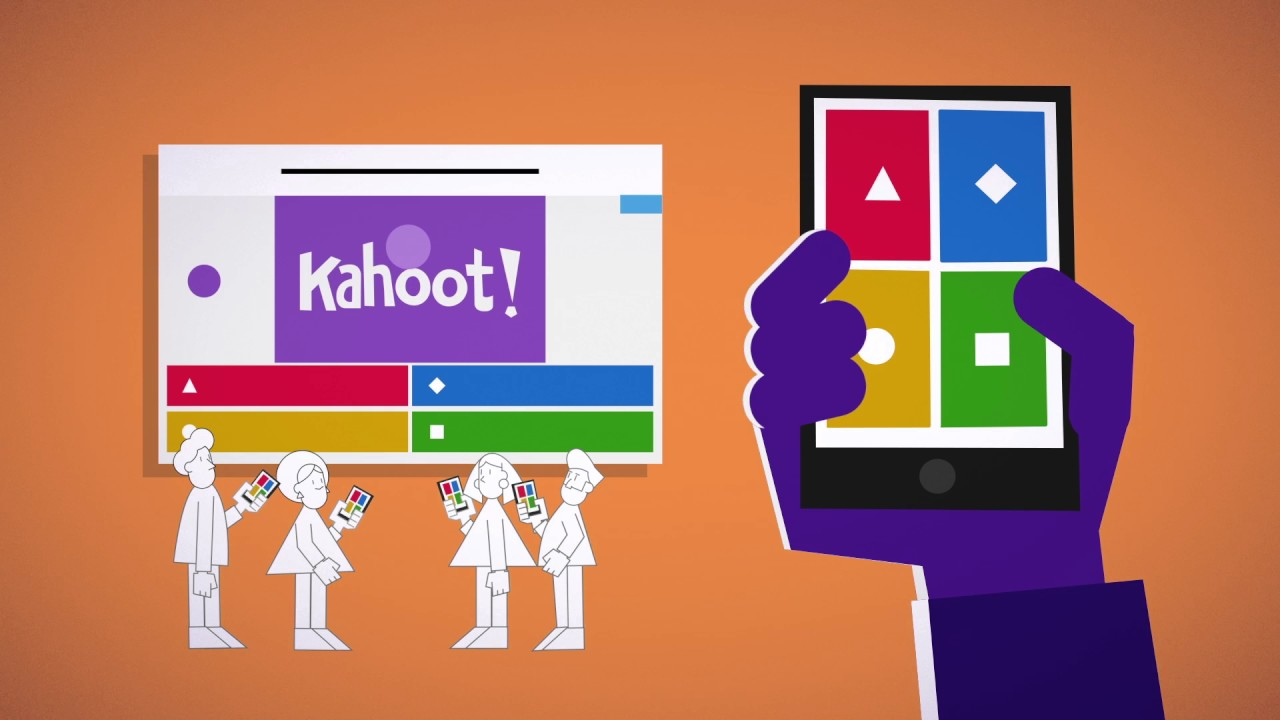
\includegraphics[width=0.8\linewidth]{figures/kahoot.jpg}
	\begin{itemize}	
	\item Using your smartphone or a second monitor
	\item Visit	\myurl{www.kahoot.it}
	\item Type the code we will give you during the class
	\end{itemize}
\end{frame}

\section{Overview to programming}
\begin{frame}{Outline}
	\tableofcontents[currentsection]
\end{frame}


\begin{frame}{What is a program?}
	\begin{itemize}
		\item A sequence of code instructions to control a machine
		\begin{itemize}
			\item Input/output
			\item Mathematical operations
			\item Conditional and repetitive executions
		\end{itemize}
		\item A recipe to instruct a machine to execute instructions. 
		\begin{itemize}
			\item We can't use a \emph{natural language}. 
			\item We need a \textbf{programming language}
		\end{itemize}
	\end{itemize}
\end{frame}

\begin{frame}{Programming languages}
	\centering
	\fbox{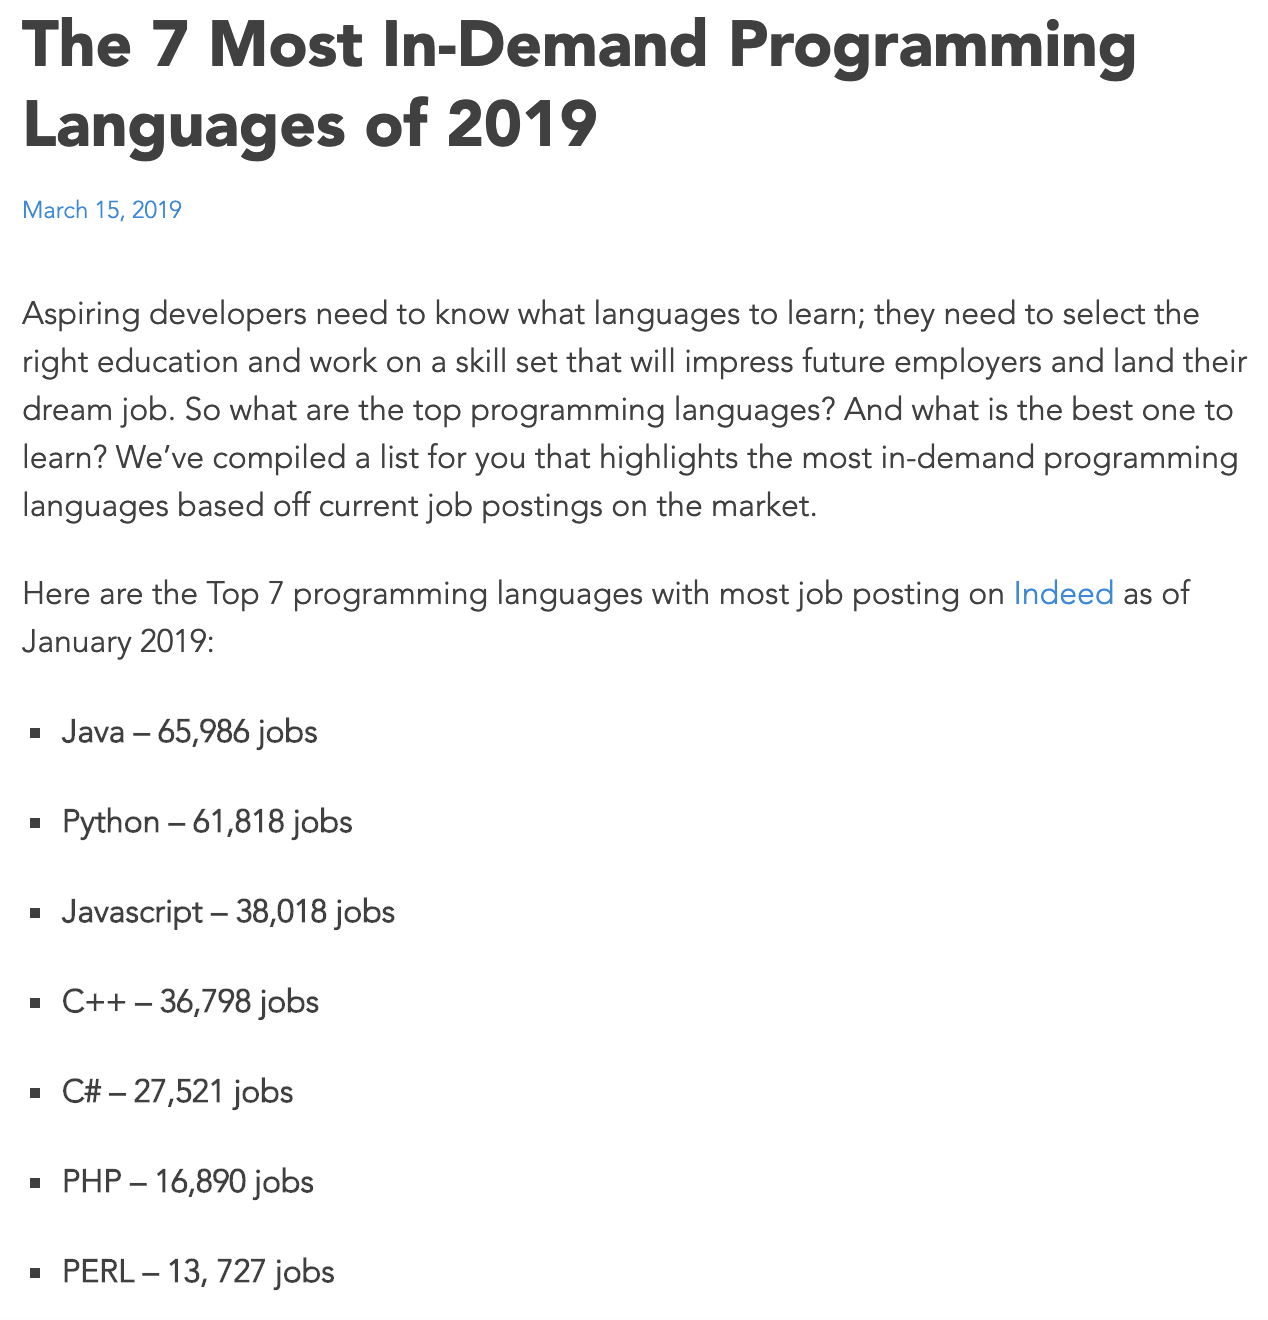
\includegraphics[width=0.45\textwidth]{figures/7mostDemanded2019}}
	\fbox{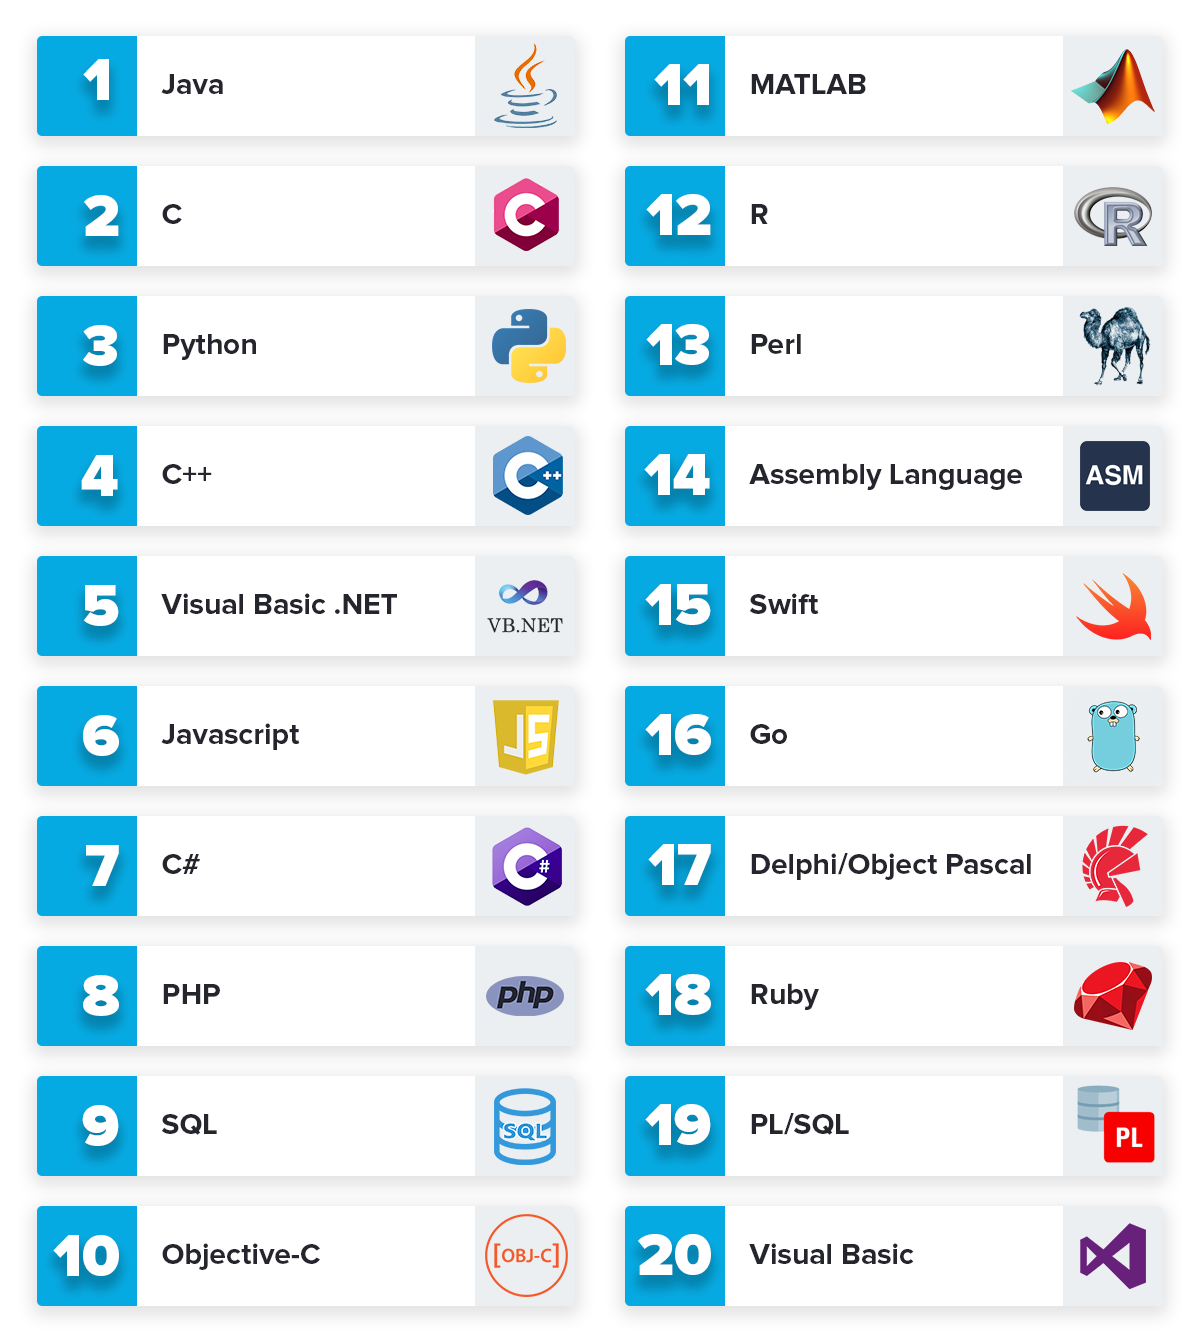
\includegraphics[width=0.45\textwidth]{figures/20mostPopularFeb2019}}
	{\scriptsize\myurl{http://www.codingdojo.com/blog/the-7-most-in-demand-programming-languages-of-2019}}
\end{frame}

\begin{frame}{Programming languages}
	%	\centering
	{\scriptsize\myurl{https://www.tiobe.com/tiobe-index/}}
	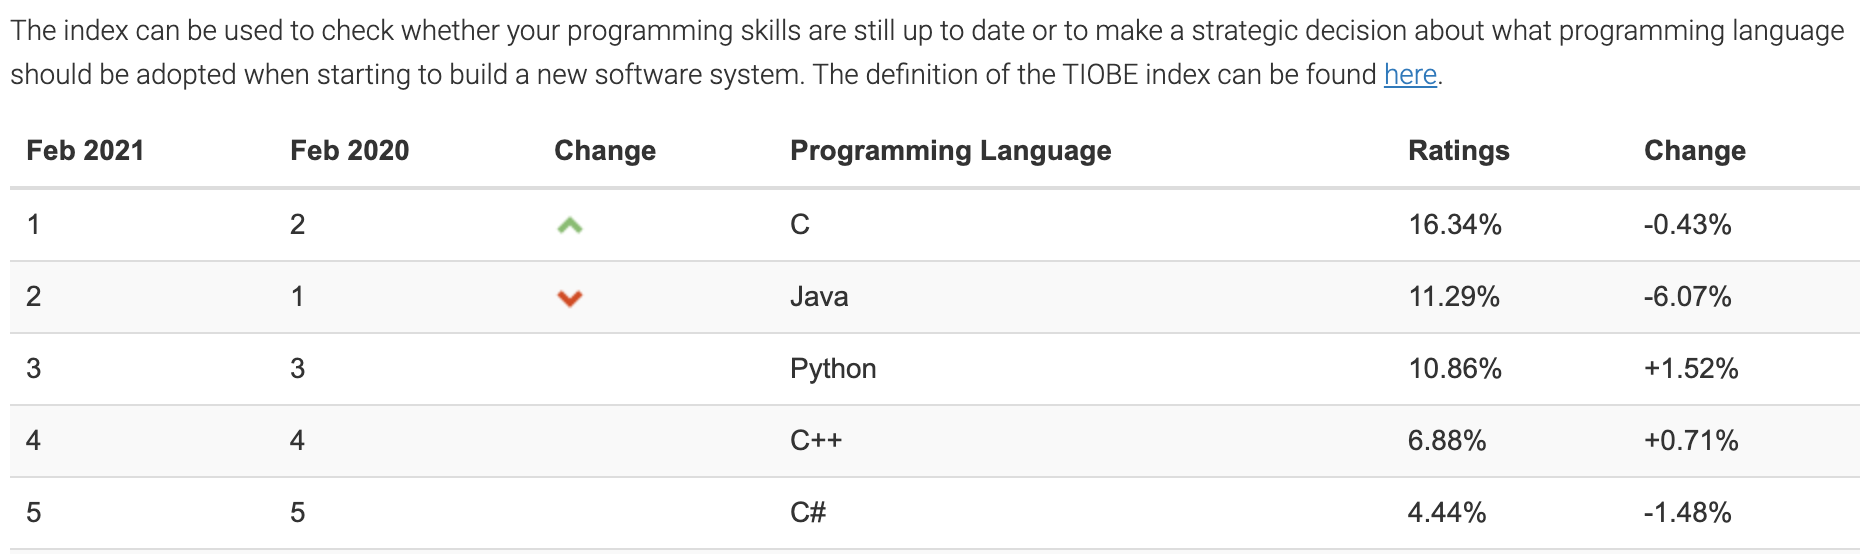
\includegraphics[scale=0.35]{figures/tiobe02_2021}\\
	\vspace{0.5cm}
	\pause
	\hspace{-0.34cm}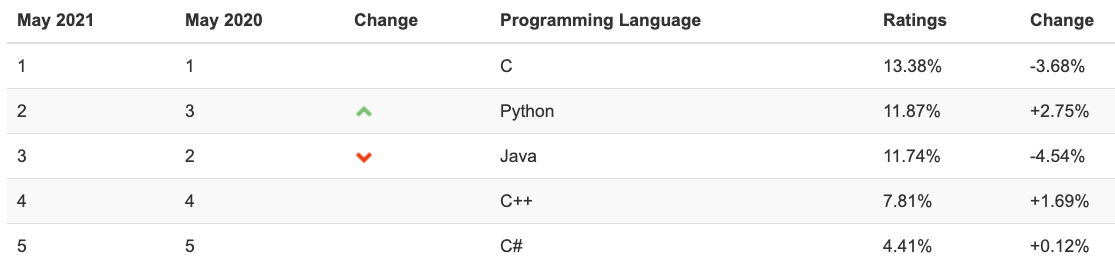
\includegraphics[scale=0.28]{figures/tiobe05_2021}
	\centering
\end{frame}

\begin{frame}{Programming languages}
		\centering
	{\scriptsize\myurl{https://www.tiobe.com/tiobe-index/}}
	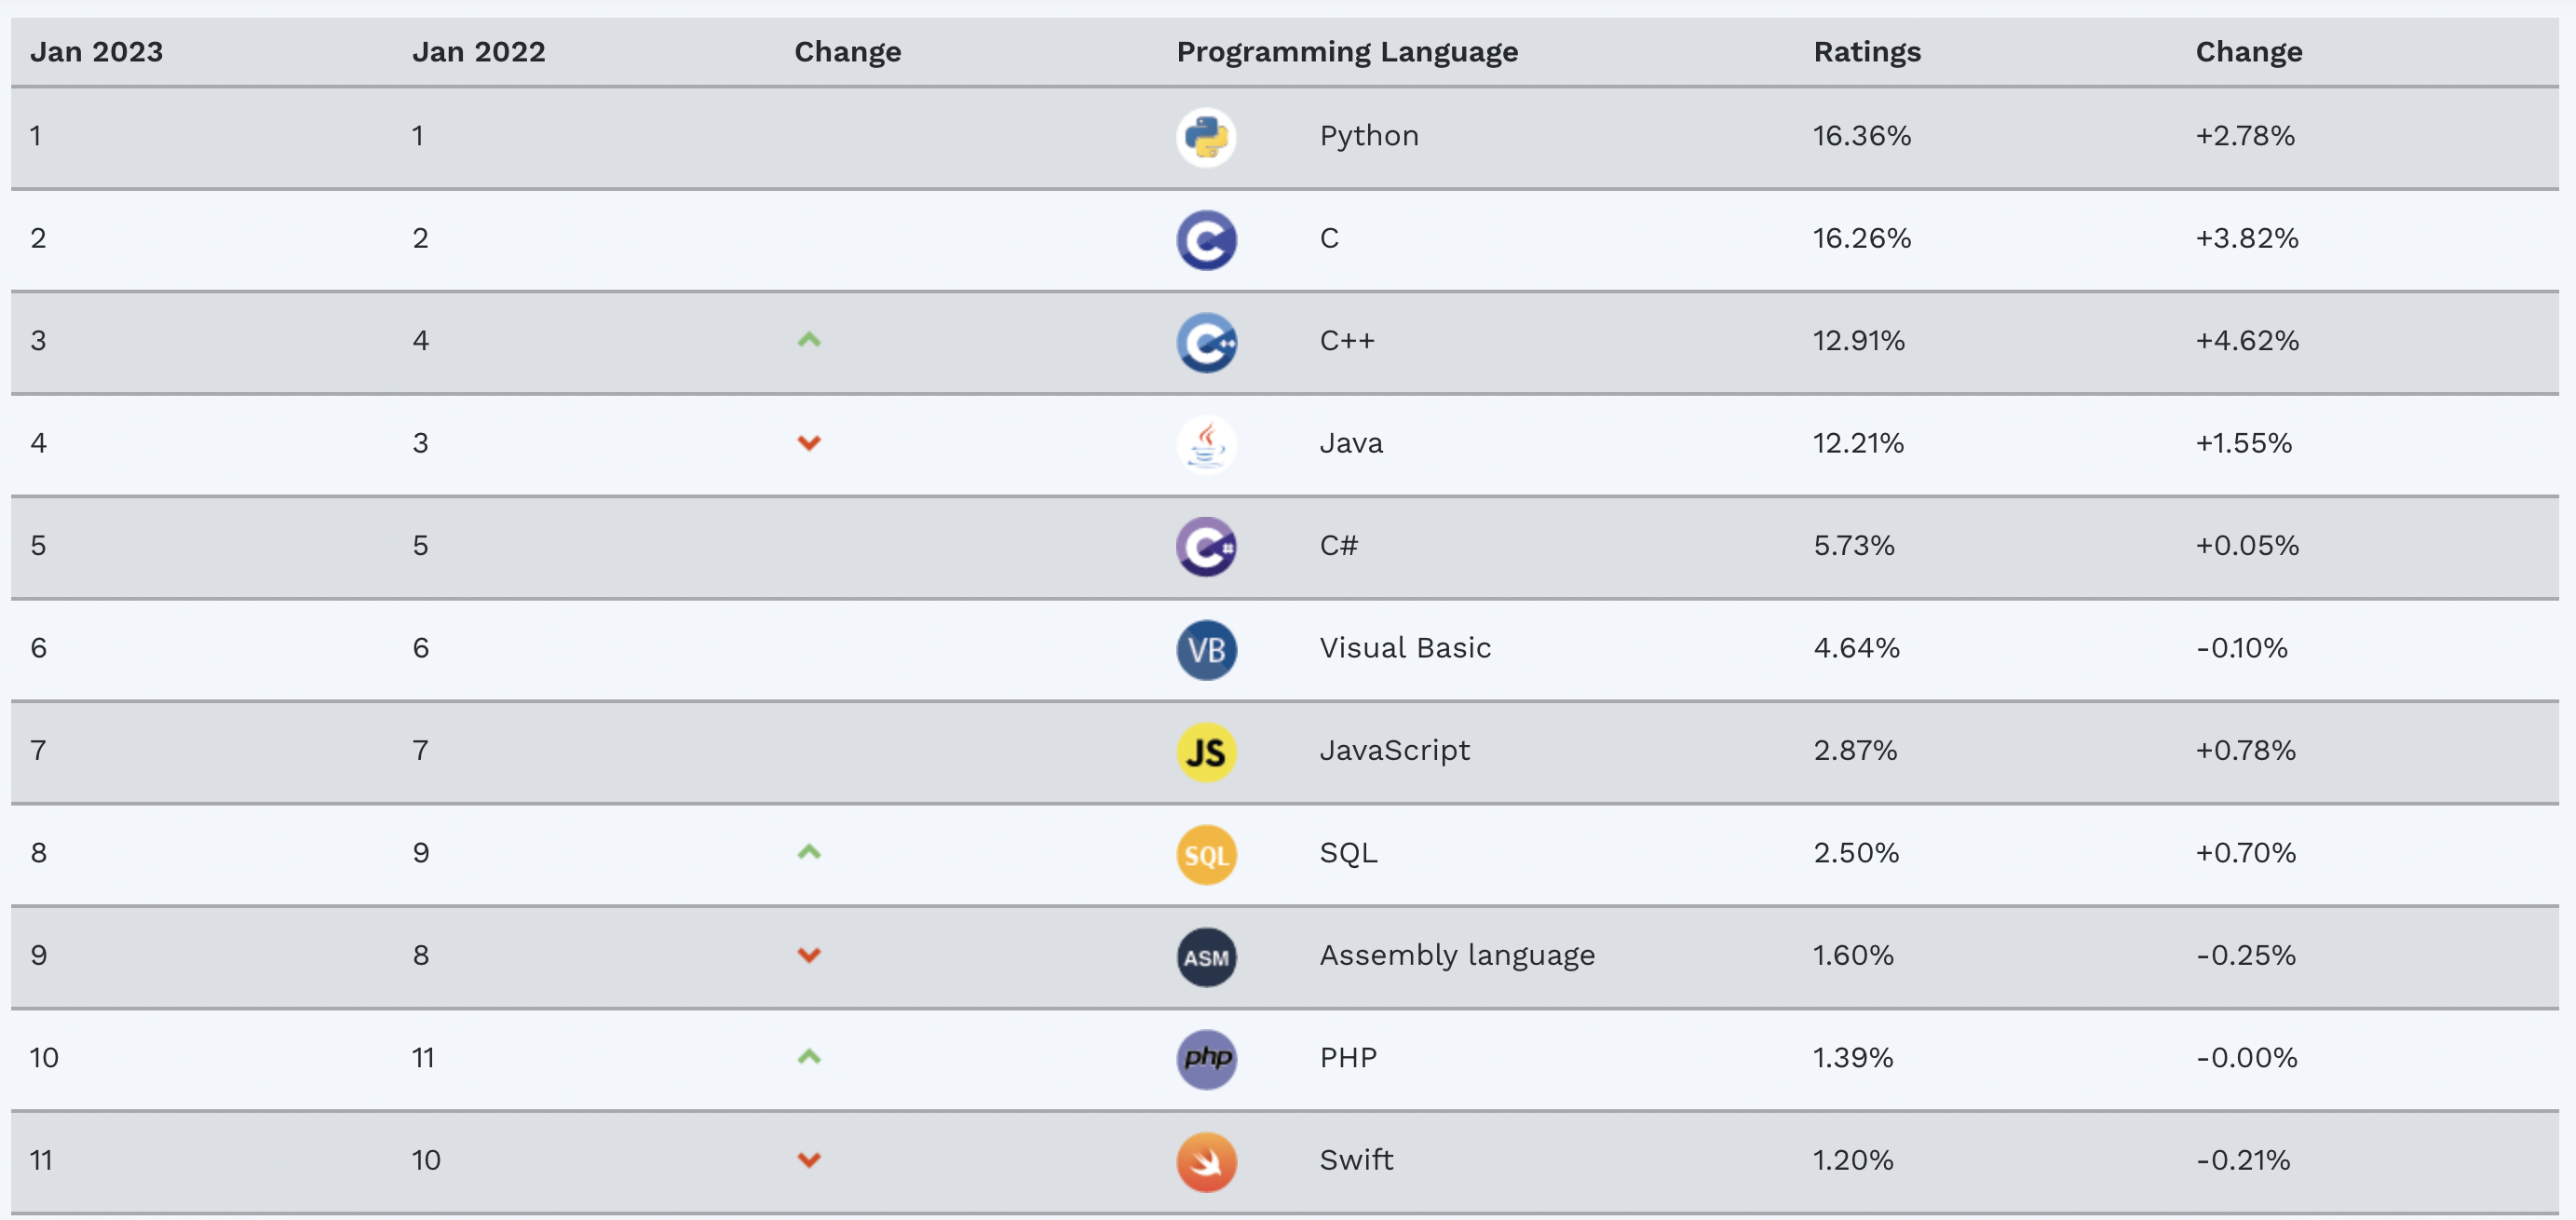
\includegraphics[scale=0.24]{figures/tiobe01_23.png}\\
\end{frame}


\begin{frame}{The Python Programming language}
	\centering
	%\begin{minipage}[t]{0.04\textwidth}
	%
\includegraphics[width=\textwidth]{figures/python-logo}
	%\end{minipage}
	
\includegraphics[width=0.1\textwidth]{figures/python-logo}
	
	%Python is a programming language
	\begin{itemize}
		\item High-level: almost human readable. Abstracts from hardware
		\item Beginner-friendly: 
		\begin{itemize}
			\item streamlined syntax
			\item it is easy to write your \emph{first programs}
		\end{itemize}	
		\item Free, open-source and multi-platform
		%\item Object-oriented: everything is an \emph{object}. This makes modularization easier. A powerful programming abstraction.
		\item Developed since the 90s, therefore it has 
		\begin{itemize}
			\item A wide community, and its popularity keeps increasing
			\item Many predefined software modules
		\end{itemize}
	\end{itemize}
\end{frame}

\begin{frame}{Python programs}
	\begin{itemize}
		\item A sequence of python instructions to control a machine
		\item Python supports the most common programming styles
		\begin{itemize}
			\item Imperative: Statements are executed in sequence changing the state of the program (the variables)
			\item Procedural: The program is structured in reusable units named functions
			\item Object-oriented: The program is structured as a collection of interacting objects that send messages to each other.
			\item {\color{gray}Functional: Statements are not written/executed as an ordered sequence of instructions. A computation is treated as the evaluation of a mathematical function.}
		\end{itemize}
	\end{itemize}
\end{frame}

\begin{frame}[fragile]
	\frametitle{{Variables}}
	\framesubtitle{Basic abstraction to represent units of data}
	A variable has a name and a value
	\begin{itemize}
		\item Names can contain any letter, number, or the underscore \_
		\\
		%\begin{minipage}{0.4\textwidth}
		%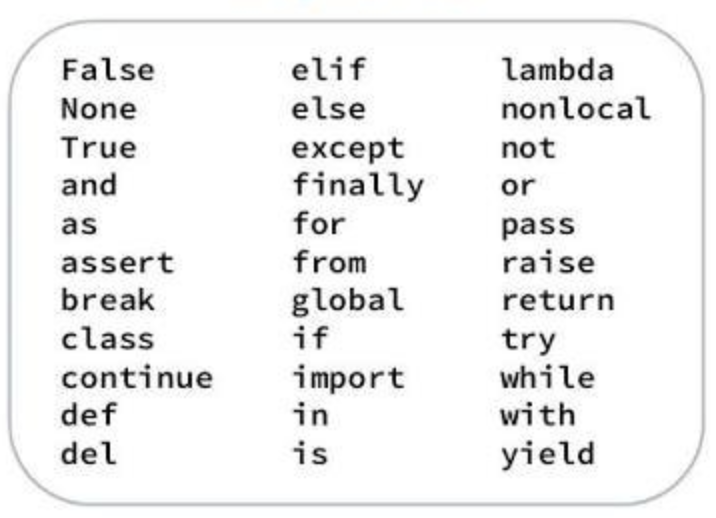
\includegraphics[width=1.0\textwidth]{figures/keywords2}
		%\end{minipage}
		\begin{minipage}{0.50\textwidth}
			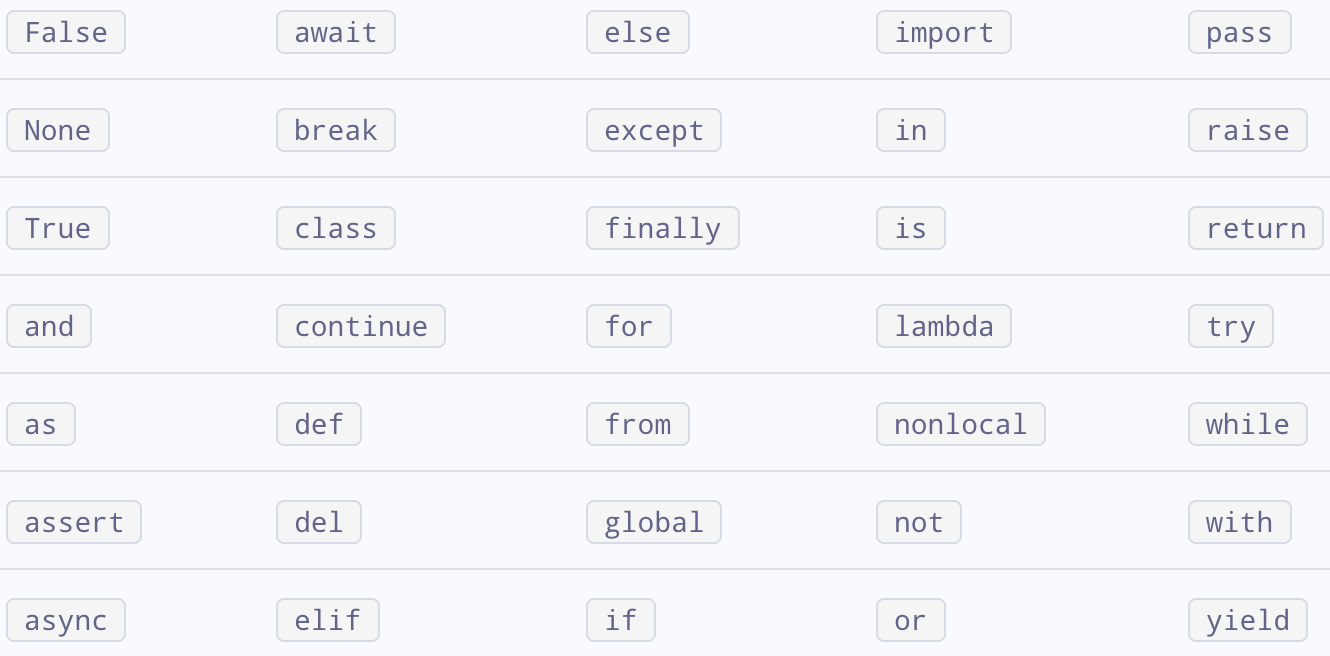
\includegraphics[width=1.0\textwidth]{figures/keywords}
		\end{minipage}
		\begin{minipage}{0.42\textwidth}
			Note:
			\begin{itemize}
				\item Cannot start with numbers
				\item Cannot be a  keyword
				\item Names are case-sensitive
			\end{itemize}
		\end{minipage}
		
		\item We assign/update values to variables using assignment statements
		%\begin{lstlisting}[language=python,basicstyle=\footnotesize\ttfamily,    stringstyle=\ttfamily\color{green}]
		
\begin{lstlisting}[language=python]
month_number=3
month_name="April"
print("The number of",month_name,"is",month_number)
month_number=4
print("The number of",month_name,"is",month_number)
\end{lstlisting}
\end{itemize}
\end{frame}

\begin{frame}{Live Programming}
\framesubtitle{Find the JupyterLab notebooks at \myurl{\homepageslides}}
\centering 
%\includegraphics[width=0.80\textwidth]{figs/live}
%\includegraphics[width=0.50\textwidth]{figs/liveCrop}
%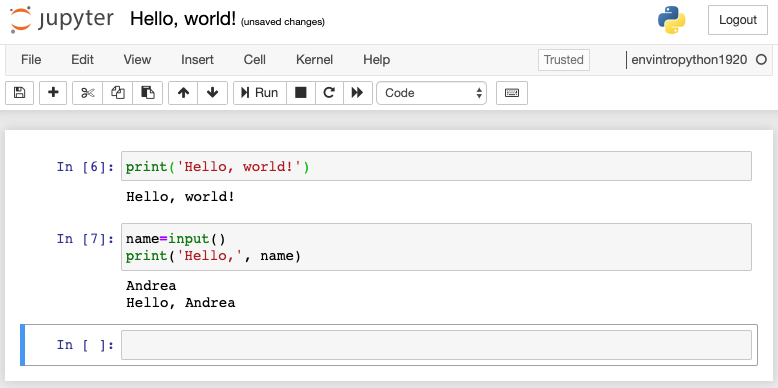
\includegraphics[width=1.0\textwidth]{figures/helloWorld}
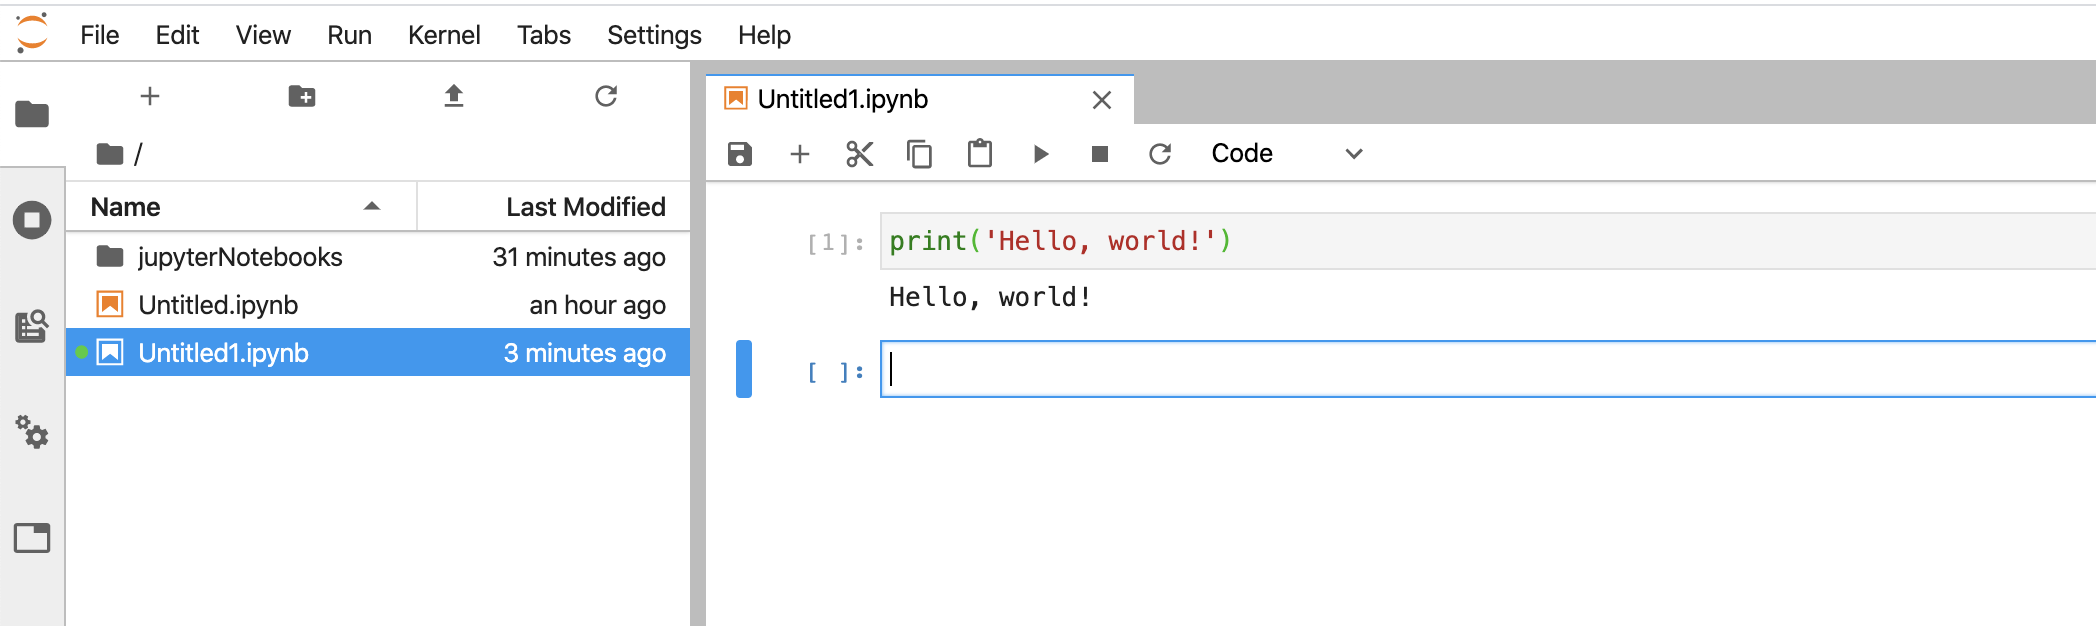
\includegraphics[width=1.0\textwidth]{figures/HelloWorldjupyterlab}
\end{frame}

\begin{frame}
	\frametitle{Configure your machine}
	\framesubtitle{If you have not done it yet}
	\centering
	Follow the instructions in\\
	\myurl{\homepagesetup}
\end{frame}

\begin{frame}{``But it works \ldots''}
	\centering 
	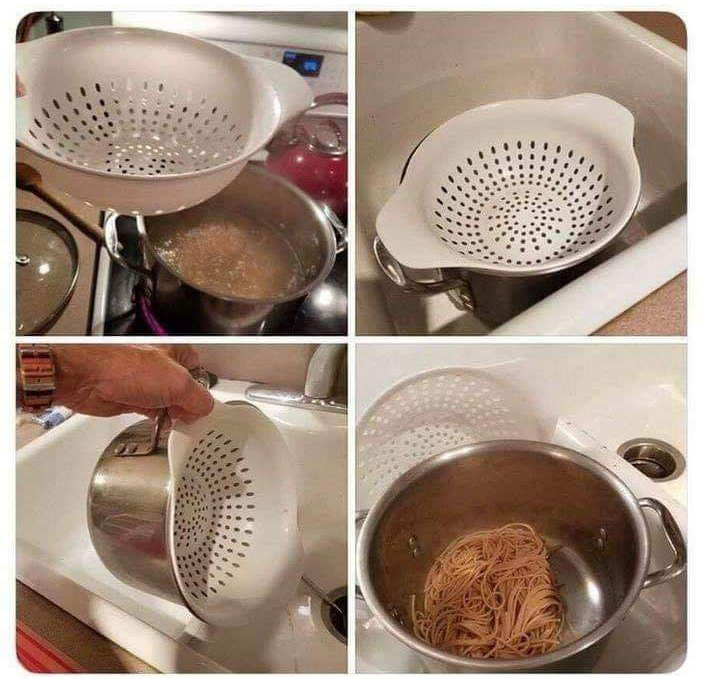
\includegraphics[width=0.7\textwidth]{figures/itDoesTheJob.jpg}
\end{frame}

\begin{frame}{``Can You Learn To Ski Without Lessons?''}
	\centering 
	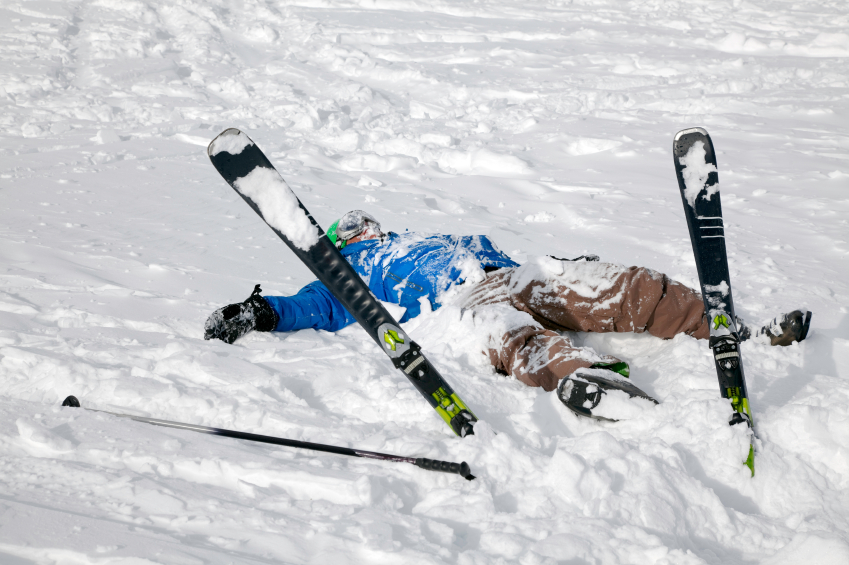
\includegraphics[width=0.7\textwidth]{figures/f737c96e-beginner-skier.jpg}
	\\
	{\scriptsize\myurl{https://www.skibro.com/blog/en/can-you-learn-to-ski-without-lessons/}}
	\\
	\vspace{0.2cm}
	%\\
	Most of the times you get to the valley. 
	\\
	\textbf{The problem is how you get there \ldots}
\end{frame}

%https://www.google.com/url?sa=i&url=https%3A%2F%2Fwww.skibro.com%2Fblog%2Fen%2Fcan-you-learn-to-ski-without-lessons%2F&psig=AOvVaw0ZUu9blkqLjpRQslcqpDFP&ust=1613575249998000&source=images&cd=vfe&ved=2ahUKEwizpIOu2u7uAhWD0-AKHcckD1AQjhx6BAgAEBI

\end{document}